\documentclass{beamer}
\mode<presentation>{
  \usetheme{Boadilla}
  \usefonttheme[onlylarge]{structurebold}
  \usefonttheme[stillsansseriflarge]{serif}
  \setbeamerfont*{frametitle}{size=\normalsize,series=\bfseries}
  \setbeamertemplate{navigation symbols}{}
  \setbeamercovered{transparent}
}
\mode<handout>{
  \usepackage{pgfpages}
  \pgfpagesuselayout{4 on 1}[a4paper,landscape,border shrink=5mm]
  \setbeamercolor{background canvas}{bg=black!10}
}
\usepackage[english]{babel}
\usepackage[latin1]{inputenc}
\usepackage{times}
\usepackage[T1]{fontenc}
\usepackage{amsmath}
\usepackage{amssymb}
\usepackage{esint}
\usepackage{hyperref}
\usepackage{tikz}
\usepackage{xkeyval}
\usepackage{xargs}
\usepackage{verbatim}
\usepackage{listings}
\usepackage{multimedia}
\usepackage{bm}
\usepackage{siunitx}
\usepackage[style=phys,citetracker=true,sorting=none,backend=bibtex]{biblatex}
\addbibresource{../library.bib}

\DeclareCiteCommand{\footfullcitetext}
[\let\thefootnote\relax\mkbibfootnotetext]
{\usebibmacro{prenote}}
{\mkbibbrackets{\thefield{labelnumber}}%
  \addnbspace%
  \usedriver
  {\DeclareNameAlias{sortname}{default}}
  {\thefield{entrytype}}}
{\multicitedelim}
{\usebibmacro{postnote}}

\makeatletter
\let\cbx@citehook=\empty
\newtoggle{cbx@blockcite}

\renewcommand{\@makefntext}[1]{%
  \noindent\normalfont\@thefnmark#1}

\DeclareCiteCommand{\sfcite}[\cbx@superscript]%
{\usebibmacro{cite:init}%
  \let\multicitedelim=\supercitedelim
  \iffieldundef{prenote}{}{\BibliographyWarning{Ignoring prenote argument}}%
  \iffieldundef{postnote}{}{\BibliographyWarning{Ignoring postnote argument}}}
{\usebibmacro{citeindex}%
  \ifciteseen
  {\ifnumequal{\value{page}}{\csuse{cbx@page@\thefield{entrykey}}}
    {}
    {\ifnumequal{\value{framenumber}}{\csuse{cbx@frame@\thefield{entrykey}}}
      {\usebibmacro{sfcite}}
      {}}}
  {\usebibmacro{sfcite}}%
  \usebibmacro{cite:comp}}
{}
{\usebibmacro{cite:dump}}

\newbibmacro*{sfcite}{%
  \csnumgdef{cbx@page@\thefield{entrykey}}{\value{page}}%
  \csnumgdef{cbx@frame@\thefield{entrykey}}{\value{framenumber}}%
  \xappto\cbx@citehook{%
    \noexpand\footfullcitetext{\thefield{entrykey}}}}

\newrobustcmd*{\cbx@superscript}[1]{%
  \mkbibsuperscript{\mkbibbrackets{#1}}%
  \iftoggle{cbx@blockcite}
  {}
  {\cbx@citehook%
    \global\let\cbx@citehook=\empty}}

\BeforeBeginEnvironment{block}{\global\toggletrue{cbx@blockcite}}

\def\metabox#1{\edef\theprevdepth{\the\prevdepth}\nointerlineskip
  \vbox to0pt{#1\vss}\prevdepth=\theprevdepth}

\AfterEndEnvironment{block}
{\metabox{%
    \global\togglefalse{cbx@blockcite}%
    \cbx@citehook%
    \global\let\cbx@citehook=\empty}}

\makeatother

\usetikzlibrary{
  arrows,
  calc,
  decorations.pathmorphing,
  decorations.pathreplacing,
  decorations.markings,
  fadings,
  positioning,
  shapes,
  arrows.meta
}
\usepgfmodule{oo}

\pgfdeclareradialshading{glow2}{\pgfpoint{0cm}{0cm}}{
  color(0mm)=(white);
  color(2mm)=(white);
  color(8mm)=(black);
  color(10mm)=(black)
}
\pgfdeclareradialshading{glow}{\pgfpoint{0cm}{0cm}}{
  color(0mm)=(white);
  color(5mm)=(white);
  color(9mm)=(black);
  color(10mm)=(black)
}

\begin{tikzfadingfrompicture}[name=glow fading]
  \shade [shading=glow] (0,0) circle (1);
\end{tikzfadingfrompicture}

\begin{tikzfadingfrompicture}[name=glow2 fading]
  \shade [shading=glow2] (0,0) circle (1);
\end{tikzfadingfrompicture}

% not mandatory, but I though it was better to set it blank
\setbeamertemplate{headline}{}
\def\beamer@entrycode{\vspace{-\headheight}}

\tikzstyle{snakearrow} = [decorate, decoration={pre length=0.1cm,
  post length=0.1cm, snake, amplitude=.4mm,
  segment length=4mm},thick, ->]

%% document-wide tikz options and styles

\tikzset{%
  % >=latex, % option for nice arrows
  inner sep=0pt,%
  outer sep=2pt,%
  mark coordinate/.style={inner sep=0pt,outer sep=0pt,minimum size=3pt,
    fill=black,circle}%
}
\tikzset{
  % Define standard arrow tip
  >=stealth',
  % Define style for boxes
  punkt/.style={
    rectangle,
    rounded corners,
    draw=black, very thick,
    text width=8em,
    minimum height=2.5em,
    text centered},
}
\makeatletter
\newbox\@backgroundblock
\newenvironment{backgroundblock}[2]{%
  \global\setbox\@backgroundblock=\vbox\bgroup%
  \unvbox\@backgroundblock%
  \vbox to0pt\bgroup\vskip#2\hbox to0pt\bgroup\hskip#1\relax%
}{\egroup\egroup\egroup}
\addtobeamertemplate{background}{\box\@backgroundblock}{}
\makeatother

% \def\timeleft{15:00->14:55}

\title{Ultracold molecule assembly}
\date{Aug 11, 2017}
\author{Yichao Yu}
\institute{Ni Group/Harvard}

\begin{document}

% Talk about cold molecule assembly experiment
% What we want to do, why we want to do it, how we do it, where we are now.
{
  \usebackgroundtemplate{
    \makebox[\paperwidth][c]{\centering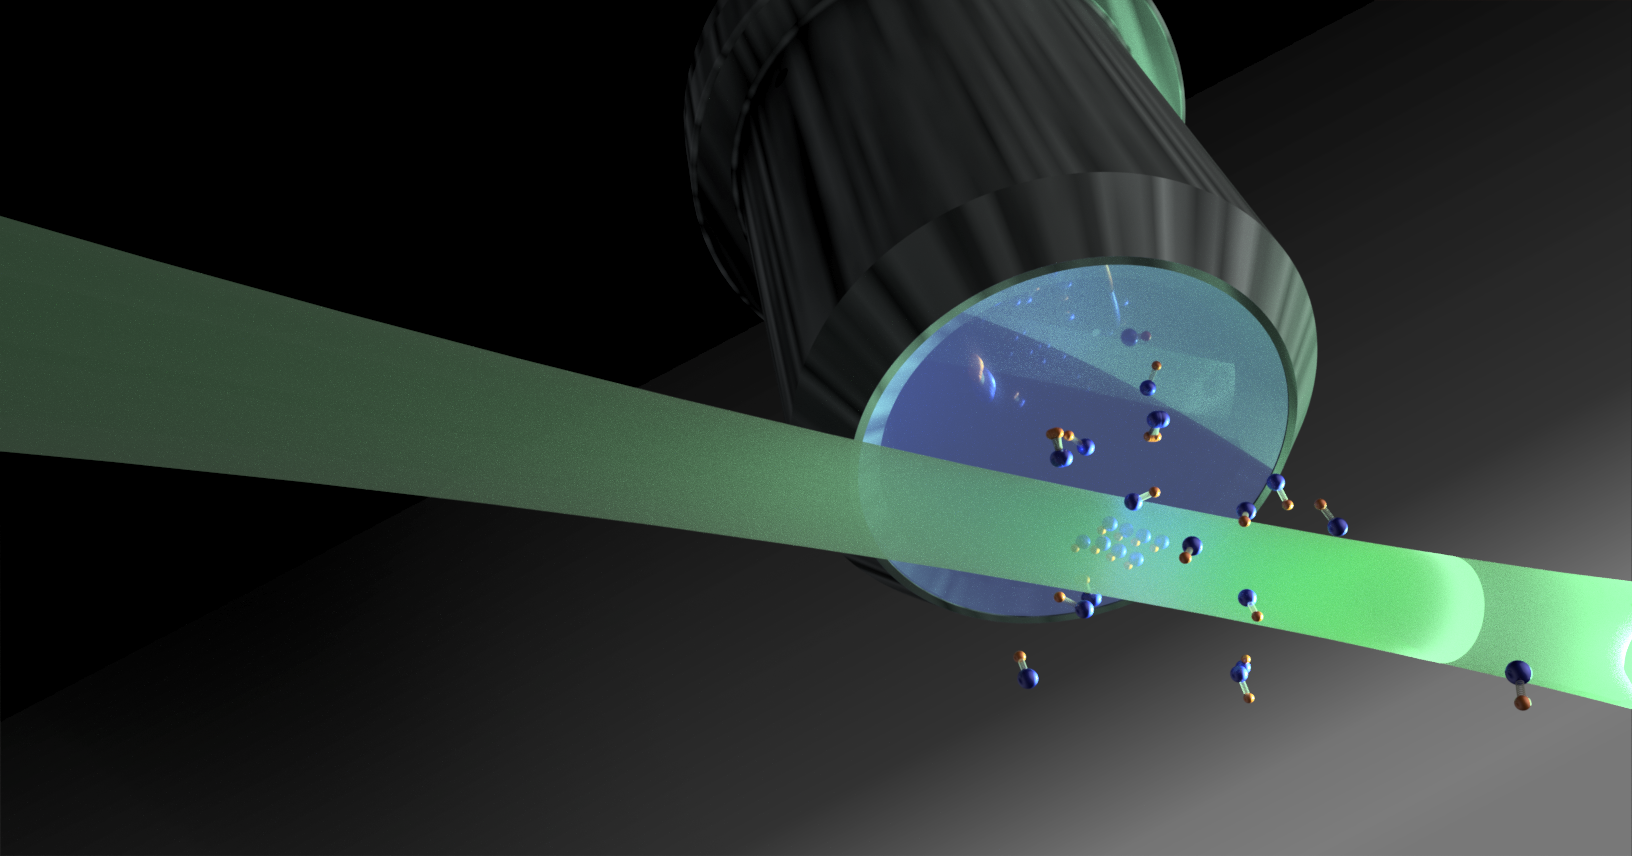
\includegraphics[height=\paperheight]{imgs/front_bg.png}}
  }
  \setbeamercolor{title}{fg=cyan!30}
  \setbeamercolor{author}{fg=white}
  \setbeamercolor{institute}{fg=white}
  \setbeamercolor{date}{fg=white}
  \begin{frame}{}
    \titlepage
  \end{frame}
}

\pgfdeclarelayer{tweezer}
\pgfsetlayers{tweezer,main}
\pgfooclass{tweezer}{
  \method tweezer() {
  }
  \method drawTweezer(#1,#2,#3) {
    \begin{pgfonlayer}{tweezer}
      \shade[shading=radial,path fading=glow fading,shift={(#1,#2)},rotate=90,yscale=1,
      fill opacity=0.9,inner color=#3]
      plot[draw,samples=200,domain=-2.5:2.5] function {sqrt(0.01 + x**2 / 10)}
      -- plot[draw,samples=200,domain=2.5:-2.5] function {-sqrt(0.01 + x**2 / 10)};
    \end{pgfonlayer}
  }
  \method drawAtom(#1,#2,#3,#4) {
    \fill [#4,path fading=glow2 fading] (#1,#2) circle (#3);
  }
  \method drawNaAtom(#1,#2,#3) {
    \pgfoothis.drawAtom(#1,#2,#3,blue);
  }
  \method drawCsAtom(#1,#2,#3) {
    \pgfoothis.drawAtom(#1,#2,#3,red);
  }
  \method drawNaTweezer(#1,#2) {
    \pgfoothis.drawTweezer(#1,#2,blue!35!black!30);
  }
  \method drawCsTweezer(#1,#2) {
    \pgfoothis.drawTweezer(#1,#2,red!30!black!30);
  }
  \method up(#1,#2) {
    \pgfoothis.drawCsTweezer(#1,#2);
    \pgfoothis.drawNaAtom(#1,#2+0.06,0.12);
    \pgfoothis.drawCsAtom(#1,#2-0.06,0.16);
  }
  \method down(#1,#2) {
    \pgfoothis.drawCsTweezer(#1,#2);
    \pgfoothis.drawCsAtom(#1,#2+0.06,0.16);
    \pgfoothis.drawNaAtom(#1,#2-0.06,0.12);
  }
  \method naTrap(#1,#2) {
    \pgfoothis.drawNaTweezer(#1,#2);
    \pgfoothis.drawNaAtom(#1,#2,0.12);
  }
  \method csTrap(#1,#2) {
    \pgfoothis.drawCsTweezer(#1,#2);
    \pgfoothis.drawCsAtom(#1,#2,0.16);
  }
}
\pgfoonew \mytweezer=new tweezer()
% The goal of our experiment:
% Create ultracold NaCs molecules that are trapped in an array of optical tweezers.
% Should have the following features
% * Strong and tunable interaction
% * Rich internal energy levels
% * High filling
% * Single site detection
% * Single site manipulation
\begin{frame}{Molecules in optical tweezer}
  \begin{columns}
    \column{4.5cm}
    \begin{block}{Features}
      \begin{itemize}
      \item<2-> Strong and tunable interaction
      \item<3-> Rich internal energy levels
      \item<4-> High filling fraction
      \item<5-> Single site detection and manipulation
      \end{itemize}
    \end{block}
    \column{7cm}
    \begin{center}
      \begin{tikzpicture}[scale=0.9]
        \mytweezer.up(0, 0)
        \mytweezer.down(2, 0.8/2.5)
        \mytweezer.up(4, 1.2/2.5)
        \begin{pgfonlayer}{tweezer}
          \draw[line width=1,dashed,color=cyan] (0, 0/2.5) -- (2, 0.8/2.5);
          \draw[line width=1,dashed,color=cyan] (0, 0/2.5) -- (1, -1.7/2.5);
          \draw[line width=1,dashed,color=cyan] (2, 0.8/2.5) -- (1, -1.7/2.5);
          \draw[line width=1,dashed,color=cyan] (3, -2.1/2.5) -- (1, -1.7/2.5);
          \draw[line width=1,dashed,color=cyan] (3, -2.1/2.5) -- (2, 0.8/2.5);
          \draw[line width=1,dashed,color=cyan] (4, 1.2/2.5) -- (2, 0.8/2.5);
          \draw[line width=1,dashed,color=cyan] (3, -2.1/2.5) -- (4, 1.2/2.5);
          \draw[line width=1,dashed,color=cyan] (3, -2.1/2.5) -- (5, -1.9/2.5);
          \draw[line width=1,dashed,color=cyan] (4, 1.2/2.5) -- (5, -1.9/2.5);
          \draw[line width=1,dashed,color=cyan] (6.2, -0.9/2.5) -- (4, 1.2/2.5);
          \draw[line width=1,dashed,color=cyan] (6.2, -0.9/2.5) -- (5, -1.9/2.5);
        \end{pgfonlayer}
        \mytweezer.down(1, -1.7/2.5)
        \mytweezer.up(3, -2.1/2.5)
        \mytweezer.down(5, -1.9/2.5)
        \mytweezer.down(6.2, -0.9/2.5)
      \end{tikzpicture}
    \end{center}
  \end{columns}
\end{frame}

% Like other ultracold atom and molecule toolboxs
% many applications that take advantage of the features

% Applications that are the most relevant
% * Quantum simulation

% ** Natural for spin model (Rich internal state that are coupled through the dipole interaction)
% ** Long range

% * Quantum computation (digital simulation)
% {* Quantum chemistry}
% {* Test for fundamental physics}
\begin{frame}{Applications}
  \begin{block}{\only<1>{\hyperlink{backup-many-body-echo}{Simulation of many-body system}\sfcite{Yan2013}}
      \only<2>{\hyperlink{backup-quantum-gate}{Quantum computation\sfcite{Yelin2006}}}}
    \hypertarget<1>{applications-many-body}{}
    \begin{center}
      \begin{tikzpicture}
        \visible<1>{
          \path (2.5, 1) node {$\displaystyle H\propto\sum \!\!V_{ij}\!\left(S_i^+S_j^-\!\!+\!S_i^-S_j^+\right)\!$};
          \path (-3.5, 0) node {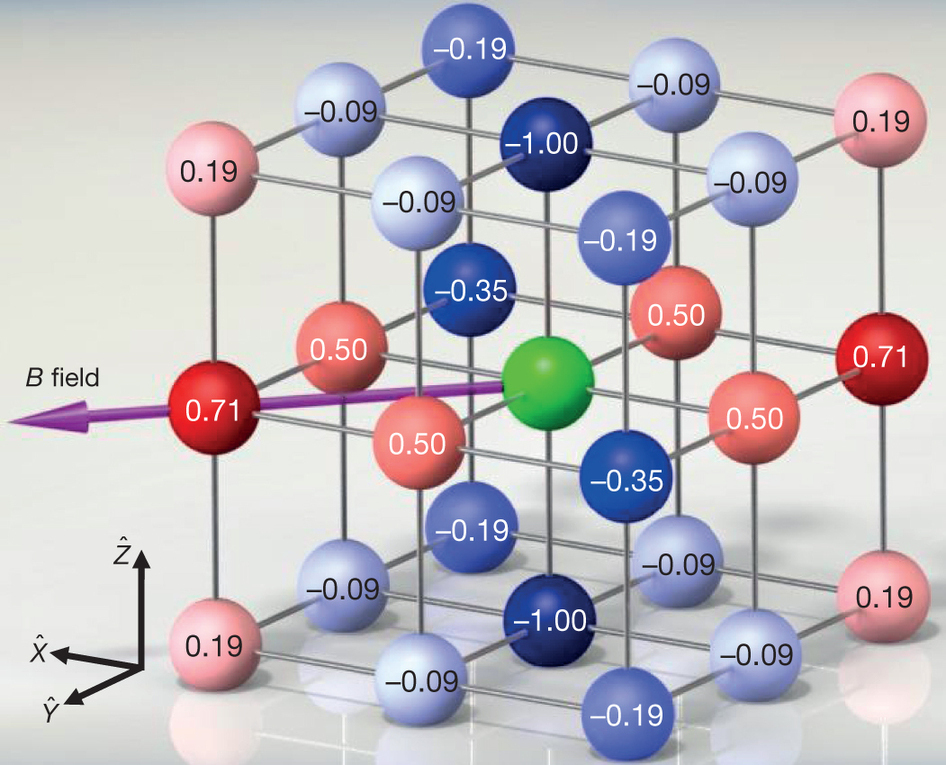
\includegraphics[width=7cm]{imgs/many-body-coupling.jpg}};
        }
        \visible<2>{
          \path (-1, 0) node {\hyperlink<2>{backup-exchange-term}{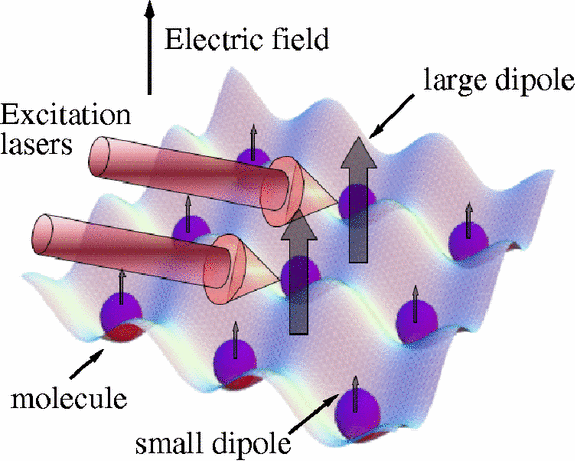
\includegraphics[width=7.5cm]{imgs/compute-geometry.png}}};
        }
      \end{tikzpicture}
    \end{center}
  \end{block}
  \hypertarget<2>{applications-quantum-gate}{}
\end{frame}

% * Use established atomic cooling techniques

% Experiment
% * MOT
% * Single atom
% * Cooling
% * Merging
% * Make molecule
\begin{frame}{Making molecules from atoms}
  \hypertarget<4>{making-molecule-rsc}{}
  \hypertarget<5>{making-molecule-merge-trap}{}
  \hypertarget<6>{making-molecule-making-molecule}{}
  \begin{columns}
    \column{4.5cm}
    \begin{itemize}
    \item<+-> MOT (Na + Cs)
    \item<+-> Loading single atoms \only<+->{}
    \item<+-> \hyperlink{raman-sideband}{Raman sideband cooling}
    \item<+-> \hyperlink{merge-trap-plan}{Merge traps}
    \item<+-> \hyperlink{backup-associate}{Make molecules!}
    \end{itemize}
    \column{8cm}
    \begin{center}
      \begin{tikzpicture}
        \begin{pgfonlayer}{tweezer}
          \fill [opacity=0,white] (-3, -3) rectangle (3, 3);
        \end{pgfonlayer}
        \only<1-2>{
          \begin{pgfonlayer}{tweezer}
            \fill [red,fill opacity=0.2,path fading=glow fading] (-0.1,0) ellipse (2.5 and 1.5);
            \fill [blue,fill opacity=0.2,path fading=glow fading] (0.1,0) ellipse (2.5 and 1.5);
          \end{pgfonlayer}{tweezer}
        }
        \only<2-4>{
          \mytweezer.drawNaTweezer(0.6, 0.0)
          \mytweezer.drawCsTweezer(-0.6, 0.0)
        }
        \only<2-3>{
          \mytweezer.drawNaAtom(0.66, 0.05, 0.27)
          \mytweezer.drawCsAtom(-0.57, 0.04, 0.22)
        }
        \only<4>{
          \mytweezer.drawNaAtom(0.6, 0.0, 0.12)
          \mytweezer.drawCsAtom(-0.6, 0.0, 0.16)
        }
        \only<5>{
          \mytweezer.drawCsTweezer(0.0, 0.0)
          \mytweezer.drawNaAtom(0.06, 0.1, 0.12)
          \mytweezer.drawCsAtom(-0.04, -0.08, 0.16)
        }
        \only<6>{
          \mytweezer.up(0, 0)
        }
      \end{tikzpicture}
    \end{center}
  \end{columns}
\end{frame}

% Current state
% * Cs more or less works as planned
\begin{frame}{Atom loading and cooling}
  \begin{columns}
    \column{5cm}
    \begin{itemize}
    \item<+-> Single atoms
    \item<+-> 85\% ground state after Cesium Raman sideband cooling
    \end{itemize}
    \column{6.5cm}
    \begin{center}
      \begin{tikzpicture}
        \visible<1>{
          \path (0, -2) node {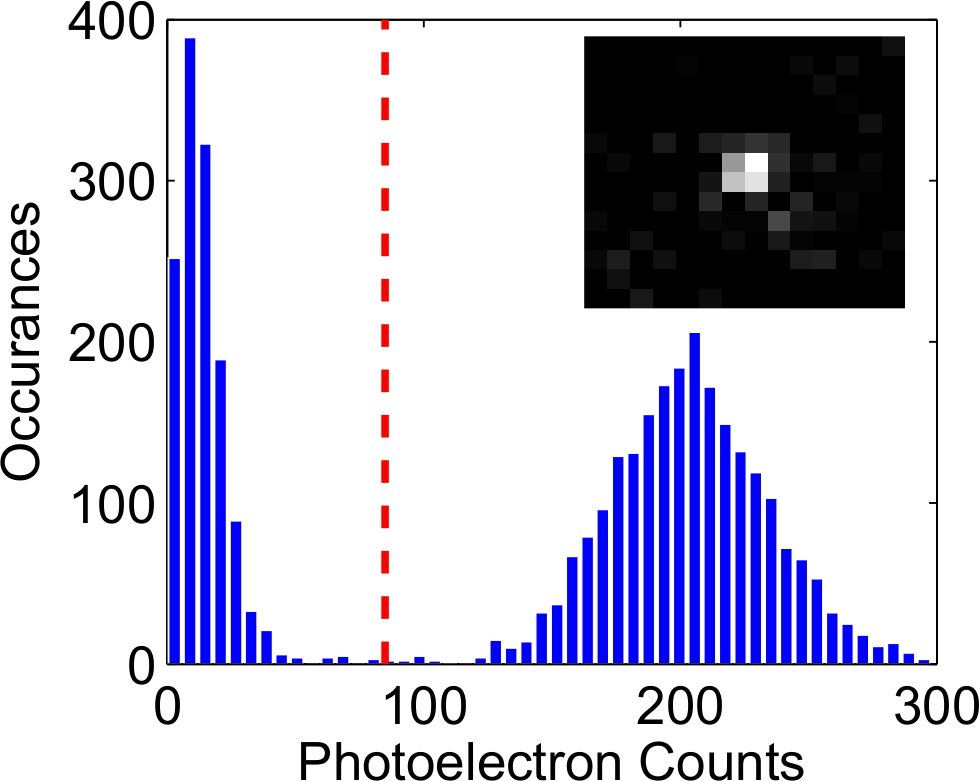
\includegraphics[width=6cm]{imgs/cs-histogram.png}};
          \path (0, 2) node
          {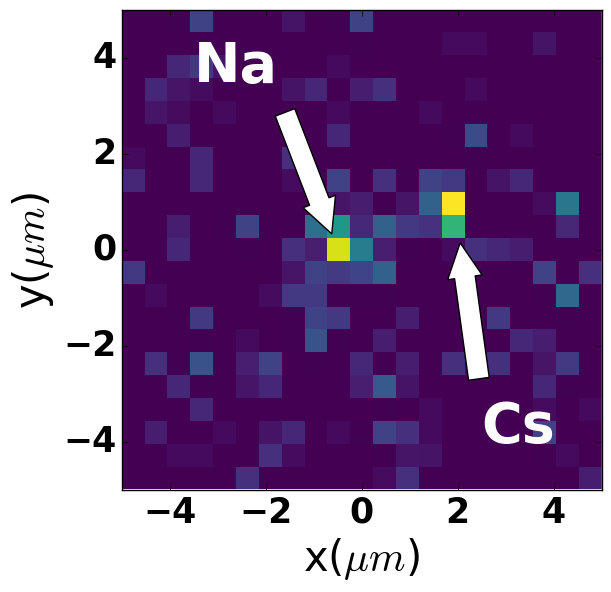
\includegraphics[width=3cm]{../../experiments/nacs_atoms/imgs/single_viridis.png}};
        }
        \visible<2>{
          \path (0, 0) node {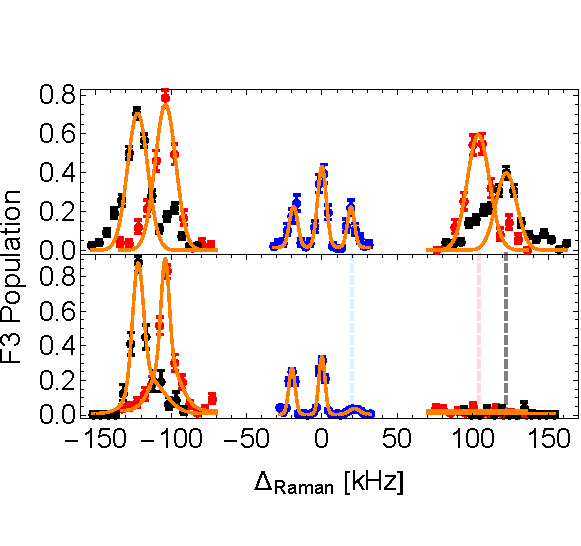
\includegraphics[width=6cm]{imgs/cs-raman-combined.pdf}};
        }
      \end{tikzpicture}
    \end{center}
  \end{columns}
\end{frame}

\begin{frame}{\hyperlink{making-molecule-rsc}{Raman sideband cooling}}
  \hypertarget<1>{raman-sideband}{}
  \begin{center}
    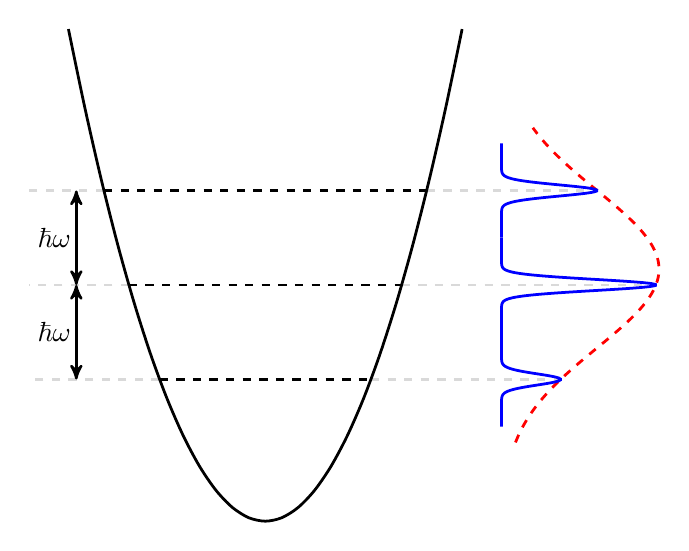
\begin{tikzpicture}
      \visible<2->{
        \draw[line width=1,red,dashed]
        plot[smooth,samples=300,domain={-2}:{2},variable=\f]
        ({2 * exp(-(\f-.2)^2/2) + 3}, {\f+3});
      }
      \foreach \y in {1.8,3,4.2} {
        \draw[line width=1,dashed,gray!30]
        ({-sqrt(\y)}, \y) -- (-3, \y);
        \draw[line width=1,dashed] ({-sqrt(\y)}, \y) -- ({sqrt(\y)}, \y);
        \visible<2->{
          \draw[line width=1,dashed,gray!30]
          ({sqrt(\y)}, \y) -- ({2 * exp(-(\y-3.2)^2/2) + 3}, \y);
          \draw[line width=1,blue]
          plot[smooth,samples=100,domain={-0.6}:{0.6},variable=\f]
          ({exp(-(\f)^2 * 100) * 2 * exp(-(\y-3.2)^2/2) + 3}, {\f+\y});
        }
      }
      \draw[<->,line width=0.9] (-2.4, 1.8) -- (-2.4, 3);
      \path (-2.4, 2.4) node[left] {$\hbar\omega$};
      \draw[<->,line width=0.9] (-2.4, 4.2) -- (-2.4, 3);
      \path (-2.4, 3.6) node[left] {$\hbar\omega$};
      \draw[line width=1]
      plot[smooth,domain={-2.5}:{2.5},variable=\x] ({\x}, {(\x)^2});
    \end{tikzpicture}
  \end{center}
\end{frame}
% Na cooling challenges
% * High initial temperature
% * High Lamb-Dicke parameter (Raman and OP)
% * Large light shift
\newcommand*{\arrowthreeD}[5]{%
  \begin{scope}[transform canvas={shift={#2}, rotate=#3}]
    \fill[left color=#1!50!black,right color=#1!50!black,middle color=#1!43,
    opacity=0.9,shading=axis,shading angle=90]
    (0,0) -- (75:#4) arc (75:105:#4) -- cycle;
    \fill[left color=#1!50!black,right color=#1!50!black,middle color=#1!43,
    opacity=0.9,shading=axis,shading angle=90]
    (84:#4) -- ++(0, #5) -- ++(-{2 * #4 * sin(6)}, 0) -- (96:#4) -- cycle;
  \end{scope}
}
\begin{frame}{}
  \begin{center}
    \begin{tikzpicture}
      \visible<1->{
        % F2 trap
        \draw[line width=1]
        plot[domain={-0.8:0.8},smooth,variable=\x] ({\x}, {(\x)^2 * 3.75 - 1});
        \foreach \y in {0.3,0.9,1.5} {
          \draw[line width=0.8] ({-sqrt(\y / 3.75)}, \y - 1) -- ({sqrt(\y / 3.75)}, \y - 1);
        }
        \path (0, 1.5 - 1) node[right,rotate=90] {\LARGE $\cdots$};

        \path (-0.5, 0.9 - 1) node[left] {$|2,-2;n\rangle$};
        \path (-0.3, 0.3 - 1) node[left] {$|2,-2;n\!\!-\!\!1\rangle$};
        \path (-1, 0.7) node[left, red!60!black] {$3^2S_{1/2}$};
      }

      \visible<1->{
        % P3/2
        \draw[line width=1] (-1, 4.3) -- (3.85, 4.3);
        \path (-1, 4.1) node[left, red!60!black] {$3^2P_{3/2}$};
      }

      \visible<2,4->{
        \draw[line width=1, densely dotted] (-1, 3.6) -- (3.85, 3.6);
        \draw[<->, line width=0.7, >=stealth] (0.75, 3.6) -- (0.75, 4.3);
        \path (0.75, 3.95) node[right] {$\Delta$};
      }

      \visible<2,4->{
        % F2 Raman
        \draw[<->, line width=0.7, >=stealth, orange] (0, 0.9 - 1) -- (0.72, 3.6);
        \path (0.55, 2.6) node[orange,above left] {$\Omega_{F2}$};
      }

      \visible<3->{
        % D2 decay
        \draw[snakearrow, >=stealth, green!70!black] (-0.4, 4.3) -- (-0.4, 0.5);
      }

      \visible<1->{
        % F1 trap
        \draw[line width=1]
        plot[domain={-0.8:0.8},smooth,variable=\x] ({\x + 2.05}, {(\x)^2 * 3.75 - 2.6});
        \foreach \y in {0.3,0.9,1.5} {
          \draw[line width=0.8] ({-sqrt(\y / 3.75) + 2.05}, \y - 2.6) -- ({sqrt(\y / 3.75) + 2.05}, \y - 2.6);
        }
        \path (2.05, 1.5 - 2.6) node[right,rotate=90] {\LARGE $\cdots$};
        \path (2.05 + 0.5, 0.9 - 2.6) node[right] {$|1,-1;n\rangle$};
        \path (2.05 + 0.33, 0.3 - 2.6) node[right] {$|1,-1;n\!\!-\!\!1\rangle$};
      }

      \visible<2,4->{
        % Raman det
        \draw[line width=0.8,densely dotted] (2.05, 0.9 - 2.6) -- (2.05 - 1, 0.9 - 2.6);
        \draw[line width=0.8,densely dotted] ({sqrt(0.4 / 3.75) + 2.05}, 0.4 - 2.6) -- (2.05 - 1, 0.4 - 2.6);
        \draw[<->, line width=0.7, >=stealth] (2.05 - 0.9, 0.9 - 2.6) -- (2.05 - 0.9, 0.4 - 2.6);
        \path (2.05 - 0.9, 0.65 - 2.6) node[right] {$\delta$};
      }

      \visible<2,4->{
        % F1 Raman
        \draw[<->, line width=0.7, >=stealth, red] (2.05, 0.4 - 2.6) -- (0.78, 3.6);
        \path (2.05 - 0.57, 0.5) node[red,right] {$\Omega_{F1}$};
      }

      \visible<1->{
        % Trap freq (F2)
        \draw[<->, line width=0.7, >=stealth] (2.05 + 0.4, 0.9 - 2.6) -- (2.05 + 0.4, 1.5 - 2.6);
        \path (2.05 + 0.4, 1.2 - 2.6) node[left] {$\omega$};
      }

      \visible<4->{
        % P1/2
        \path (1.2, 2.85) node[above right, red!60!black] {$3^2P_{1/2}$};
        \draw[line width=1] (1.7, 2.85) -- (3.35, 2.85);

        \draw[->, line width=0.7, >=stealth, blue] (3.15, 0.6) -- (3.15, 2.85);
        \draw[->, line width=0.7, >=stealth, blue] (3.5, -1.5) -- (3.5, 4.3);
        \path (3.5, 2.5) node[right, blue] {$\Gamma_{OP}$};
      }

      \visible<3>{
        % P1/2
        \path (-1, 3.5) node[left, red!60!black] {$3^2P_{1/2}$};
        \draw[line width=1] (-1, 3.5) -- (3.35, 3.5);

        \draw[->, line width=0.7, >=stealth, blue] (3.15, 0.6) -- (3.15, 3.5);
        \draw[->, line width=0.7, >=stealth, blue] (3.5, -1.5) -- (3.5, 4.3);
        \path (3.5, 2.5) node[right, blue] {$\Gamma_{OP}$};
        % D1 decay
        \draw[snakearrow, >=stealth, green!70!black] (0.4, 3.5) -- (0.4, 0.5);
      }

      \pgfmathsetmacro{\radiush}{0.75}
      \pgfmathsetmacro{\theight}{2}
      \pgfmathsetmacro{\radiusv}{.7 * \radiush}
      \pgfmathsetmacro{\waist}{.15}
      \pgfmathsetmacro{\xscale}{\radiush / sqrt(1 + (\waist)^2)}
      \pgfmathsetmacro{\trapcenterx}{7}
      \pgfmathsetmacro{\trapcentery}{3}

      \begin{scope}[transform canvas={shift={(\trapcenterx, \trapcentery)}}]
        \fill[left color=red!50!black,right color=red!50!black,middle color=red!43,shading=axis,
        rotate={-45},shading angle=32]
        plot[domain={-1}:{1}, smooth, variable=\y]
        ({sqrt((\y)^2 + (\waist)^2) * \xscale}, {\y * \theight})
        arc (0:180:\radiush cm and \radiusv cm)
        -- plot[domain={-1}:{1}, smooth, variable=\y]
        ({-sqrt((\y)^2 + (\waist)^2) * \xscale}, -\y * \theight)
        arc (180:360:\radiush cm and \radiusv cm);
        \visible<2,4->{
          \begin{scope}[transform canvas={rotate={4}}]
            \arrowthreeD{orange}{(0.3, 0)}{-90}{0.3}{2};
            \path (1.7, 0) node[above,orange!80!black] {Raman F2};
          \end{scope}
          \draw[->,>=stealth,line width=1,color=black!60] (4:2.5) -- ++ (90-30:0.25);
          \draw[->,>=stealth,line width=1,color=black!60] (4:2.5) -- ++ (90-30:-0.3);
          \draw[orange!50!black, <->, densely dotted, >=stealth, line width=0.6]
          (3:2.2) arc (3:-30:2.2 and 1.2);
          \path (-8:2.3) node[orange!50!black, right] {$42^\circ$};
          \draw[->,>=stealth,line width=1,color=black!60]
          (-1.95, -0.25+1.95*0.28) arc (-90:60:0.15 and 0.25);
        }
        \visible<3->{
          \draw[line width=1,color=black!60] (1.3, -0.25-1.3*0.28) arc (-90:60:0.15 and 0.25);
        }
        \begin{scope}[transform canvas={cm={1,-0.28,0,1,(0, 0)}}]
          \visible<2,4->{
            \draw[->,>=stealth,line width=1,color=black!60]
            (-0.25, 1.05) arc (180:35:0.25 and 0.15);
            \draw[line width=1,color=black!60] (-0.25, -1.05) arc (180:35:0.25 and 0.15);
          }
          \draw[blue, dotted, line width=0.5] (0, 0) -- (2.0, 0);
          \fill[blue!50!black,opacity=0.1] (-2.2, 1.65) rectangle (1.8, -1.6);
          \draw[blue!50!black, densely dotted,line width=0.6] (-2.2, 1.65) rectangle (1.8, -1.6);
          \visible<2,4->{
            \arrowthreeD{red}{(0, -0.2)}{180}{0.3}{1};
            \arrowthreeD{orange}{(-0.2, 0)}{90}{0.3}{1.65};
            \arrowthreeD{red}{(0, 0.2)}{0}{0.3}{1};
            \path (-1, 0) node[above,orange!80!black] {Raman F2};
            \path (0, 1.3) node[left,red!80!black,align=center] {Raman F1};
            \path (0, -1.3) node[right,red!80!black,align=center] {Raman F1};
          }
          \visible<3->{
            \arrowthreeD{cyan!40!blue}{(0.2, 0)}{-90}{0.3}{1.1};
            \path (0.8, 0) node[below,cyan!20!blue!80!black] {OP};
          }
          \visible<2->{
            \draw[white,opacity=0.5,->,>=stealth,line width=1] (1.61, 1.49) -- (0.36, 1.49);
            \draw[->,>=stealth,line width=1] (1.6, 1.5) -- (0.35, 1.5);
            \path (1.01, 1.49) node[below,white,opacity=0.5] {B field};
            \path (1.0, 1.5) node[below] {B field};
          }
          \visible<2,4->{
            \draw[line width=1,color=black!60] (-0.25, 1.05) arc (180:330:0.25 and 0.15);
            \draw[->,>=stealth,line width=1,color=black!60]
            (-0.25, -1.05) arc (180:330:0.25 and 0.15);
          }
        \end{scope}
        \visible<3->{
          \draw[->,>=stealth,line width=1,color=black!60]
          (1.3, -0.25-1.3*0.28) arc (-90:-240:0.15 and 0.25);
        }
        \visible<2,4->{
          \draw[line width=1,color=black!60]
          (-1.95, -0.25+1.95*0.28) arc (-90:-250:0.15 and 0.25);
        }
        \fill[left color=red!50!black,right color=red!50!black,middle color=red!43,
        shading=axis,rotate=-45,shading angle=40]
        plot[domain={-1}:{0}, smooth, variable=\y] ({sqrt((\y)^2 + (\waist)^2) * \xscale}, \y * \theight)
        arc (0:180:{(\radiush)*(\waist)} and {(\radiusv)*(\waist)})
        -- plot[domain={0}:{1}, smooth, variable=\y] ({-sqrt((\y)^2 + (\waist)^2) * \xscale}, -\y * \theight)
        arc (180:360:\radiush cm and \radiusv cm);
        \fill[red!50!gray,rotate=-45]
        ({-sqrt(1 + (\waist)^2) * \xscale}, -\theight*1.05)
        arc (180:{360+180}:\radiush cm and \radiusv cm);
      \end{scope}

      \visible<4,9->{
        \fill[white, opacity=0.35] (-2.22, 5.25) rectangle (9.9, -2.7);
      }
      \node[right, color={frametitle.fg}] at (-2.2, 5)
      {\textbf{Raman sideband cooling}};
      \visible<5-8>{
        \fill[white, opacity=0.97] (-2.22, 5.25) rectangle (9.9, -2.7);
      }
      \visible<5>{
        \node[below right] at (-2.4, 5.2) {\includegraphics[width=6cm]{imgs/op_branching_1.pdf}};
      }
      \visible<6-8>{
        \node[below right] at (-2.4, 5.2) {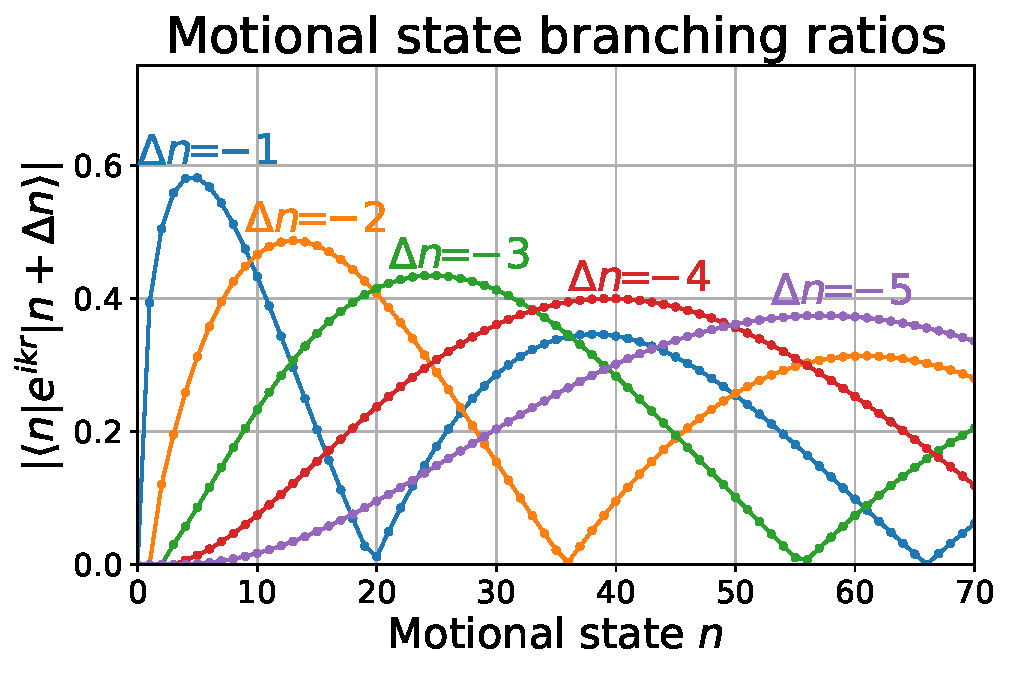
\includegraphics[width=6cm]{imgs/op_branching.pdf}};
      }
      \visible<7-8>{
        \node[above right] at (-2.3, -3.5) {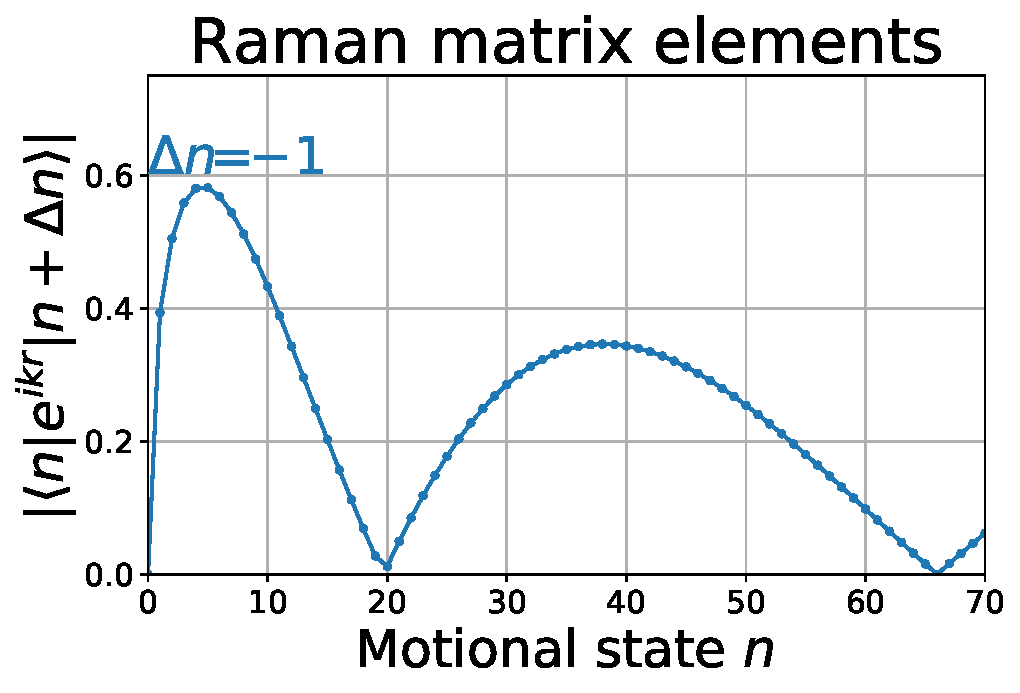
\includegraphics[width=6cm]{imgs/mele_raman_1.pdf}};
      }
      \visible<8>{
        \hypertarget<8>{raman-difficulty-pdf}{}
        \node[below left] at (9.9, 5.5) {\hyperlink<8>{backup-diff-adiabatic}{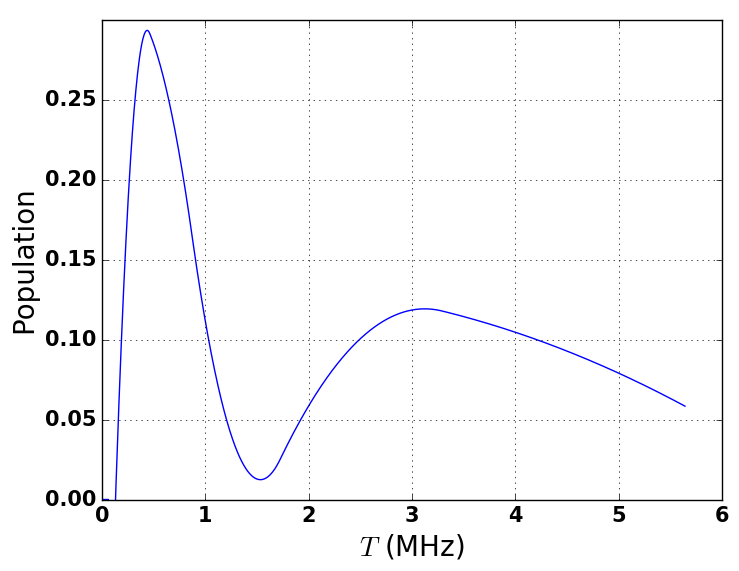
\includegraphics[width=6cm]{../../experiments/adiabatic_lowering/imgs/AC_old-pulsed_pdf.png}}};
      }

      \visible<4->{
        \node[text width=6cm,above right,align=center] at (4, -3.0) {
          \begin{itemize}
          \item<4-> High initial temperature ($70\mu K$)
          \item<5-> High Lamb Dicke parameter\\
            $\eta\equiv kz_0$
          \item<9-> Large light shift
          \item<10-> Trap anharmonicity
          \item<11-> Off resonance scattering
            $\approx3\sim15$kHz
          \end{itemize}
        };
      }
    \end{tikzpicture}
  \end{center}
\end{frame}

% * Simulation
\begin{frame}{Sequence and simulation}
  \begin{center}
    \begin{tikzpicture}
      \visible<1> {
        \path (0, 0) node {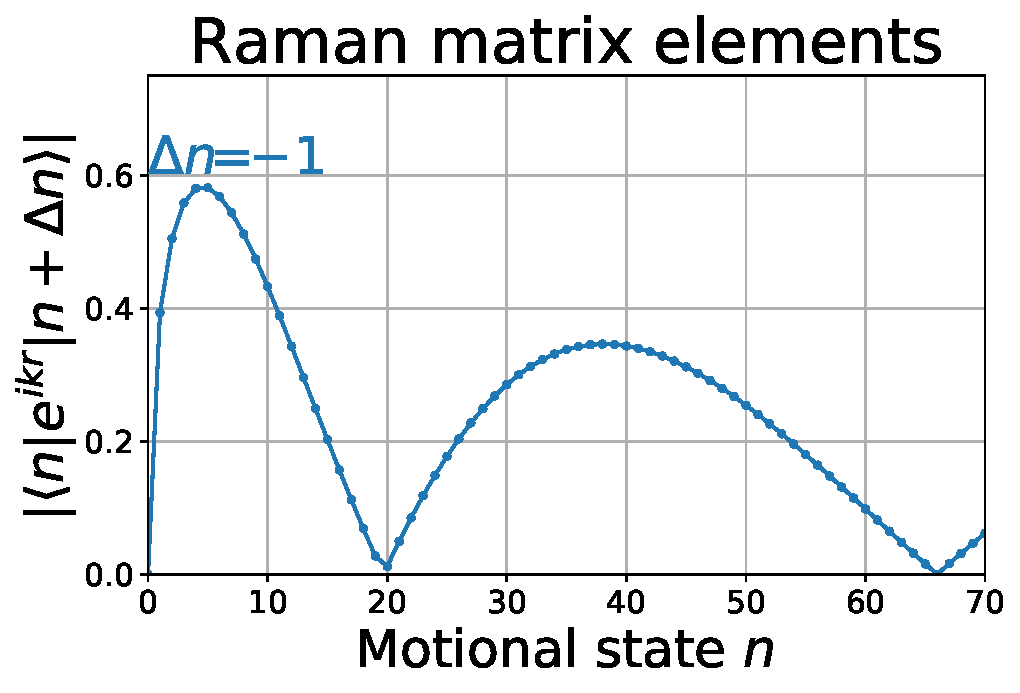
\includegraphics[width=10cm]{imgs/mele_raman_1.pdf}};
      }
      \visible<2> {
        \path (0, 0) node {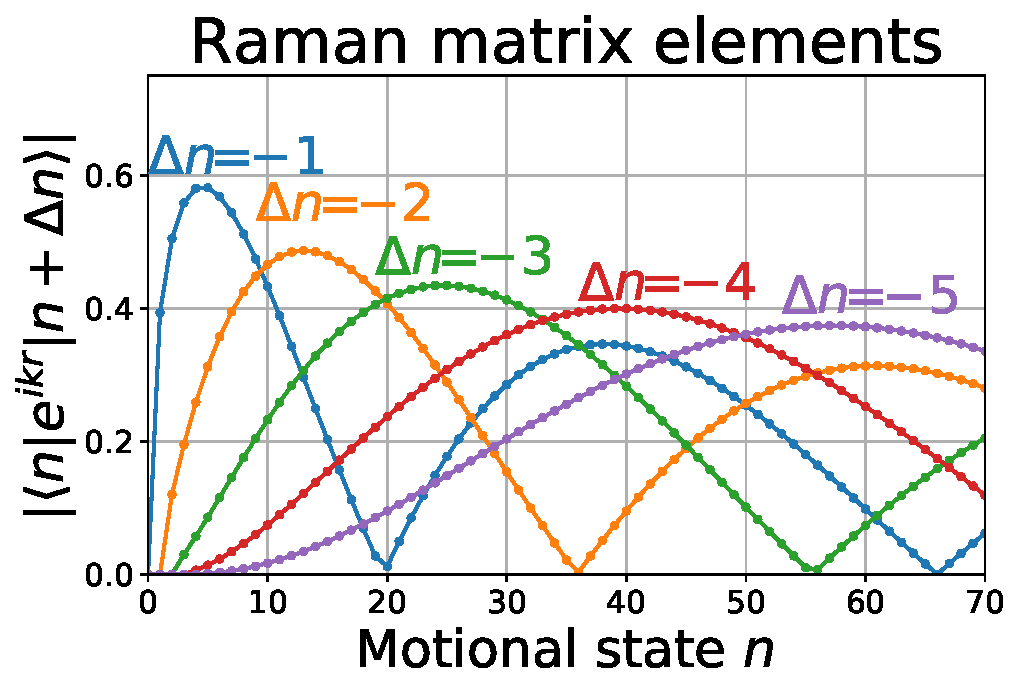
\includegraphics[width=10cm]{imgs/mele_raman.pdf}};
      }
      \visible<3> {
        \path (0, 0) node {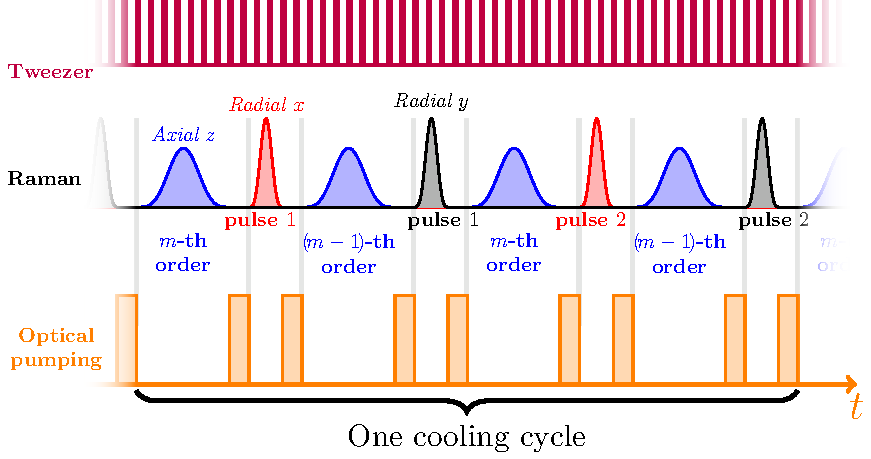
\includegraphics[width=12cm]{sequence.pdf}};
      }
      \visible<4> {
        \path (0, 0) node {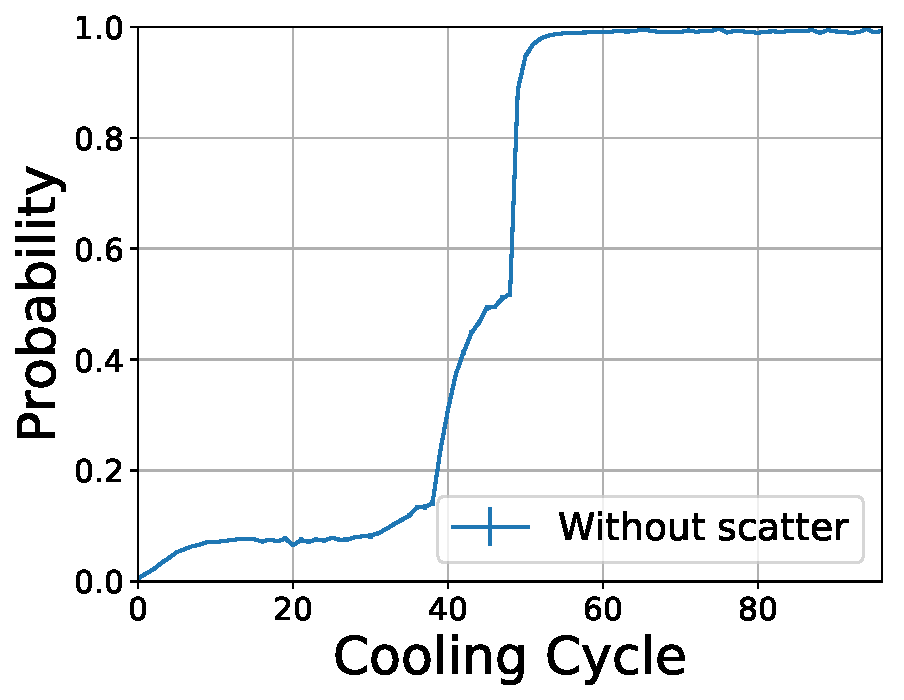
\includegraphics[width=10cm]{imgs/simcool_no_scatter.pdf}};
      }
      \visible<5> {
        \path (0, 0) node {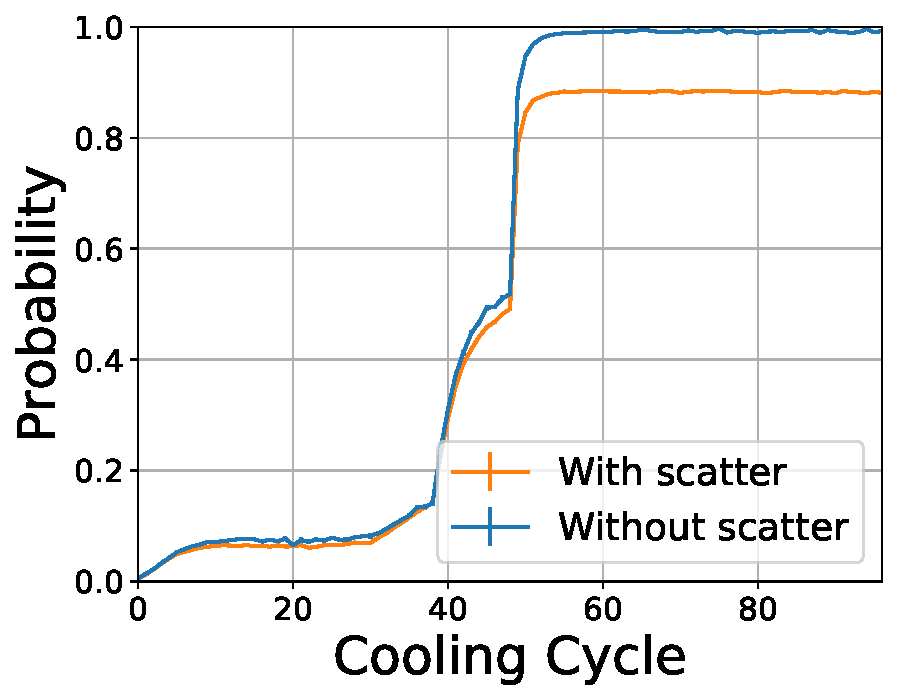
\includegraphics[width=10cm]{imgs/simcool_real.pdf}};
      }
    \end{tikzpicture}
  \end{center}
\end{frame}

% * Result
\begin{frame}{Raman sidebands}
  \begin{center}
    \begin{tikzpicture}
      \visible<1> {
        \path (0, 0) node {
          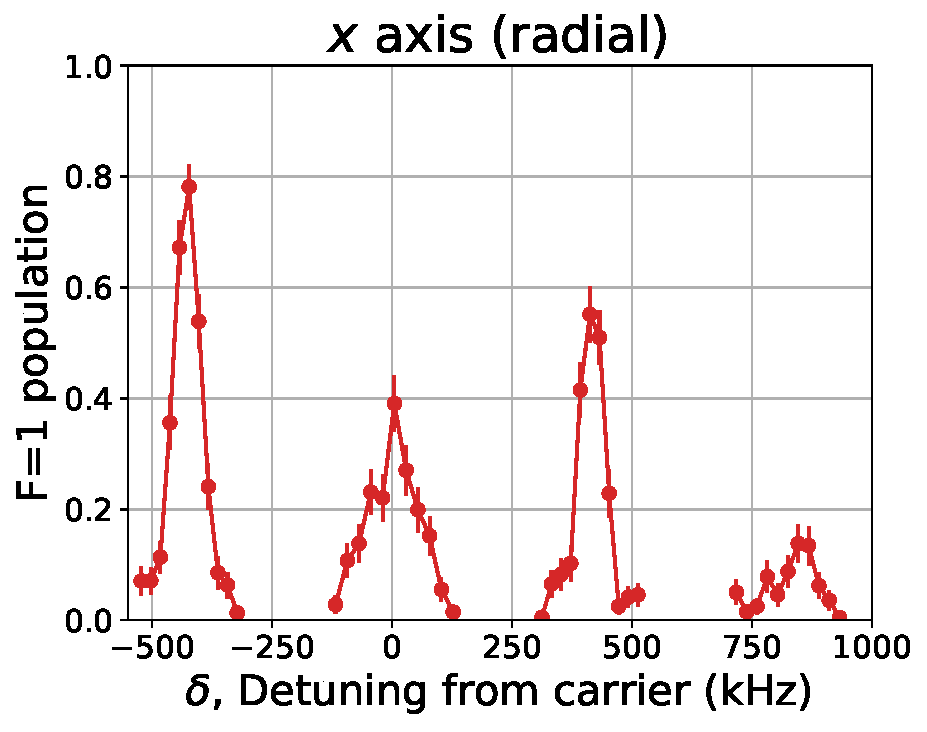
\includegraphics[width=10cm]{imgs/spectrum_r2_init.pdf}
        };
        \draw[<-, line width=1.5] (-0.7, 0) -- (0, 1.6) node[right] {\Large Carrier};
      }
      \visible<2> {
        \path (0, 0) node {
          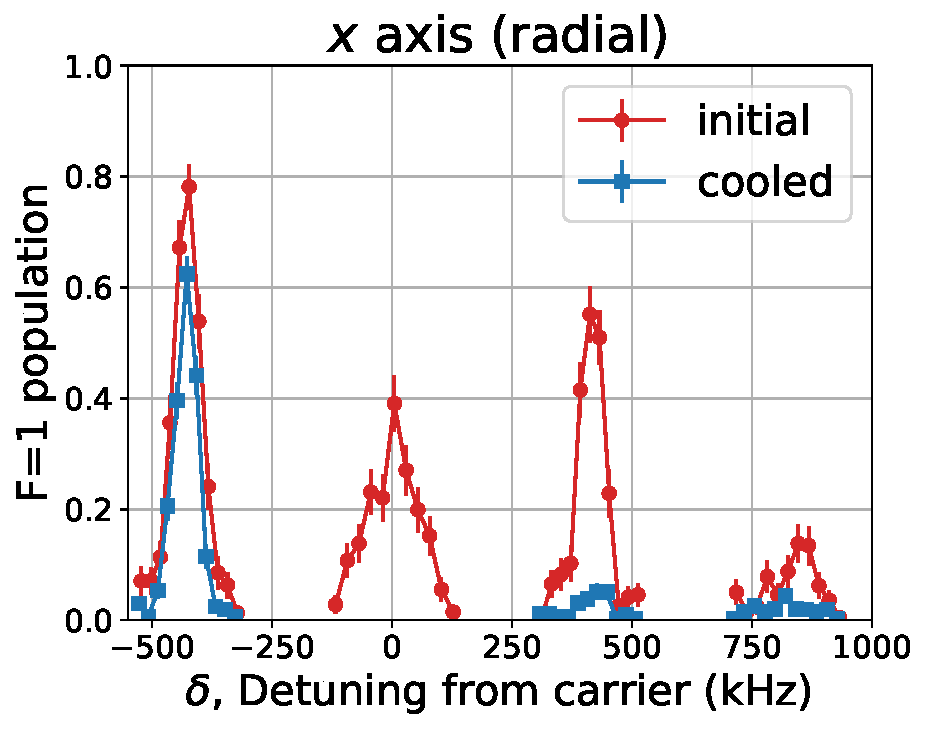
\includegraphics[width=10cm]{imgs/spectrum_r2.pdf}
        };
      }
      \visible<3> {
        \path (0, 0) node {
          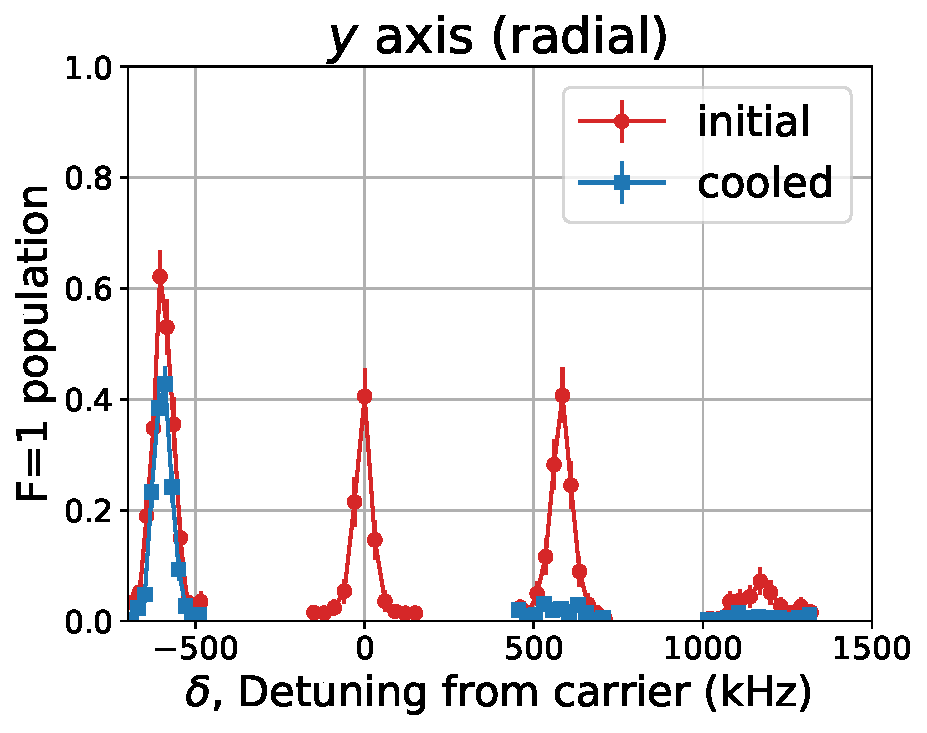
\includegraphics[width=10cm]{imgs/spectrum_r3.pdf}
        };
      }
    \end{tikzpicture}
  \end{center}
\end{frame}

\begin{frame}{Raman sidebands}
  \begin{center}
    \begin{tikzpicture}[scale=1.41176]
      \visible<1> {
        \path (0, 0) node {
          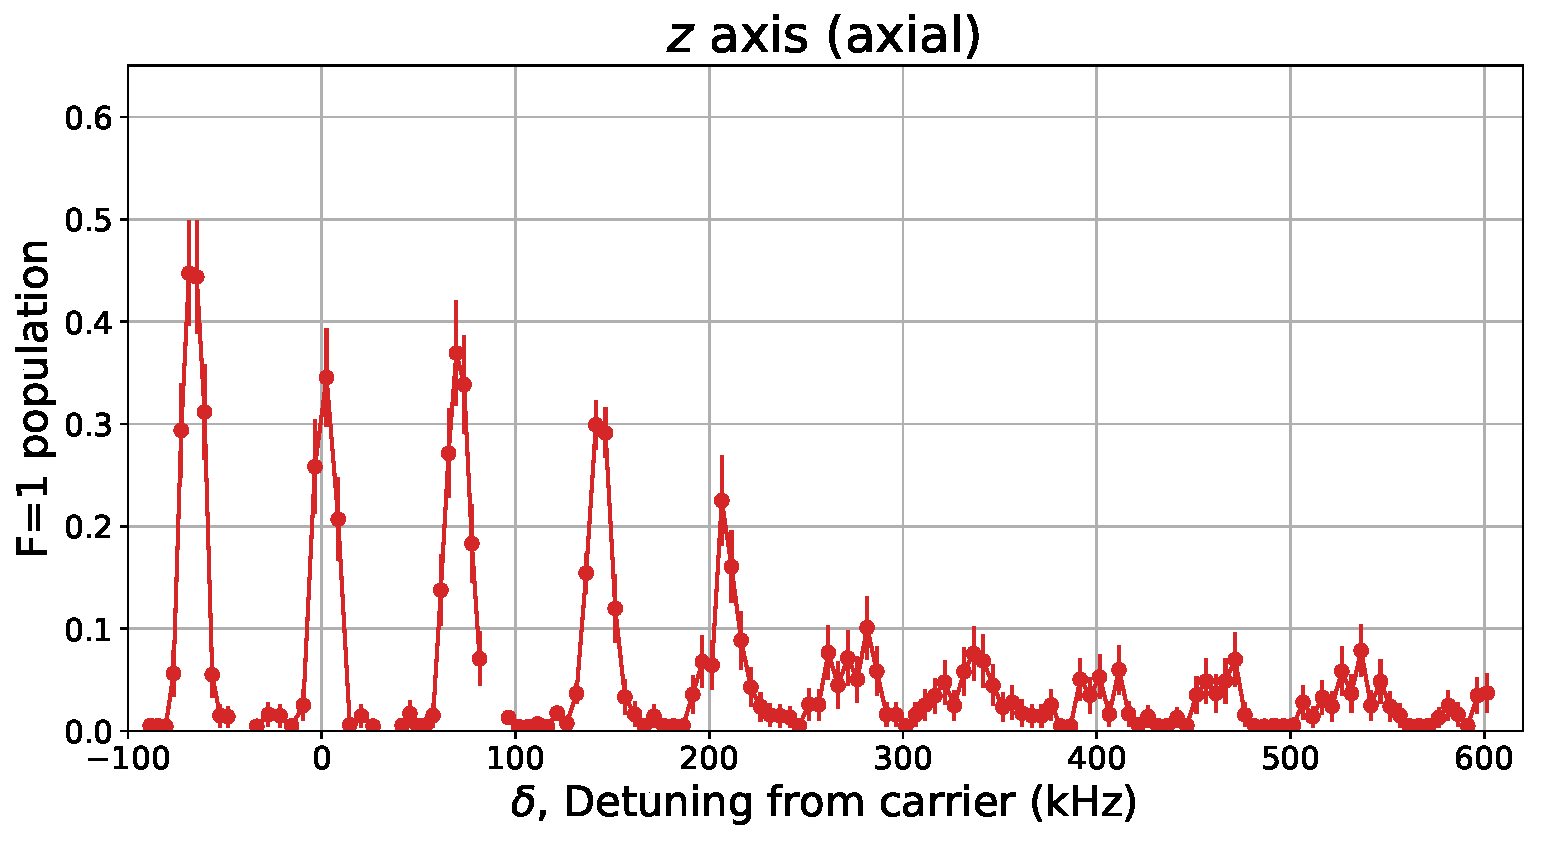
\includegraphics[width=12cm]{imgs/spectrum_a1_init.pdf}
        };
        \draw[red, <-, line width=1.5] (-3.15, 0.75) -- (-2.95, 1.2)
        node[above right] {\Large 1st order heating};
        \draw[<-, line width=1.5] (-2.45, 0.25) -- (-2.25, 0.8) node[above right] {\Large Carrier};
        \draw[black!40!green, <-, line width=1.5] (-1.7, 0.23) -- (-1.55, 0.6)
        node[right] {\Large 1st order cooling};
        \draw[blue, <-, line width=1.5] (-0.95, -0.05) -- (-0.55, 0.1)
        node[right] {\Large 2nd order cooling};
        \path[magenta] (0.25, -0.5) node[right] {\Large And higher orders{$\cdots$}};
      }
      \visible<2-> {
        \path (0, 0) node {
          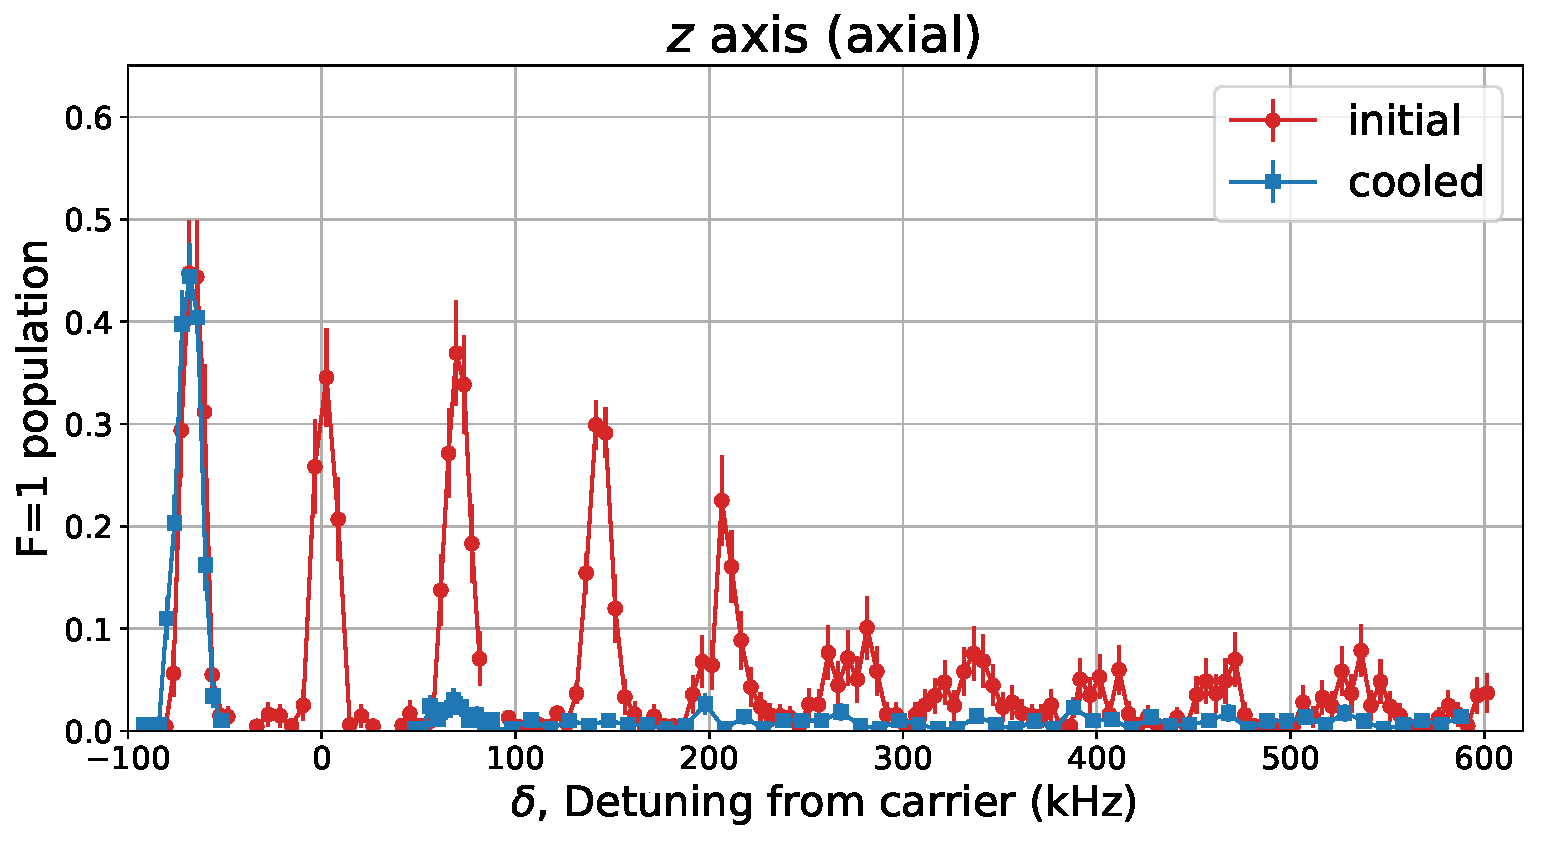
\includegraphics[width=12cm]{imgs/spectrum_a1.pdf}
        };
      }
      \visible<3-> {
        \fill[white,opacity=0.95] (-4.2, -2.5) rectangle (5, 2.5);
        \path (0, 1) node[align=center]
        {
          \begin{tabular}{|c|c|}
            \hline
            \textbf{Axis}&\textbf{Ground state probability}\\\hline
            $x$ (Radial)&92(2)\%\\\hline
            $y$ (Radial)&95(2)\%\\\hline
            $z$ (Axial)&93(3)\%\\\hline
          \end{tabular}
        };
        \visible<4-> {
          \path (0, -1) node[align=center]
          {
            \textbf{3D ground state:} $81(4)\%$\\
            \textbf{Loss after cooling:} $15\%$\\\\
            \textbf{Total 3D ground state preparation fidelity:} $69(3)\%$
          };
        }
      }
    \end{tikzpicture}
  \end{center}
\end{frame}

\begin{frame}{Rabi flopping (radial)}
  \begin{center}
    \begin{tikzpicture}
      \node[above] at (0, 0) {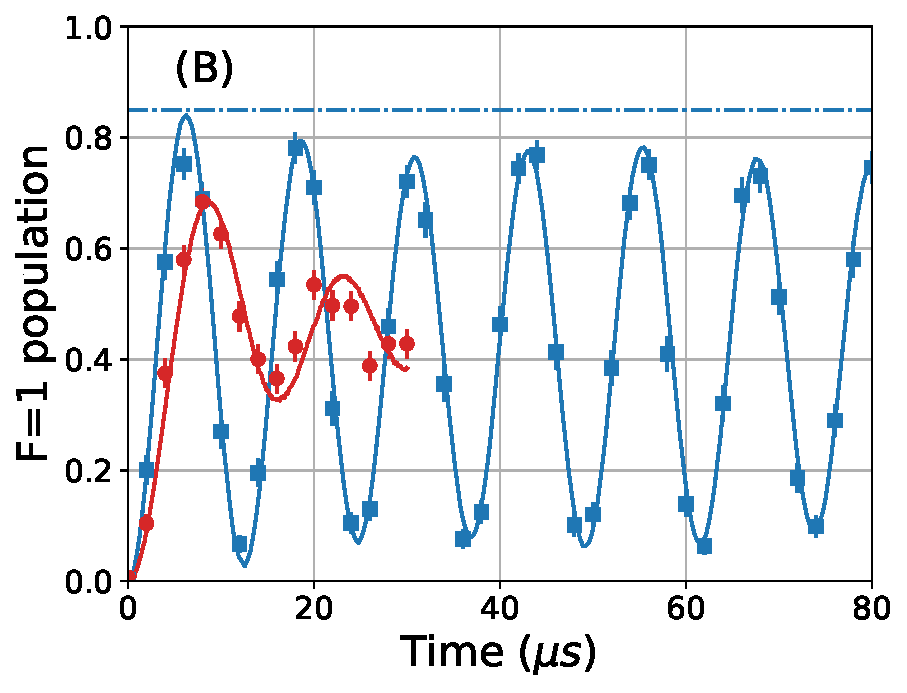
\includegraphics[width=6cm]{imgs/rabi_flop_r2_0.pdf}};
      \node[above] at (6, 0) {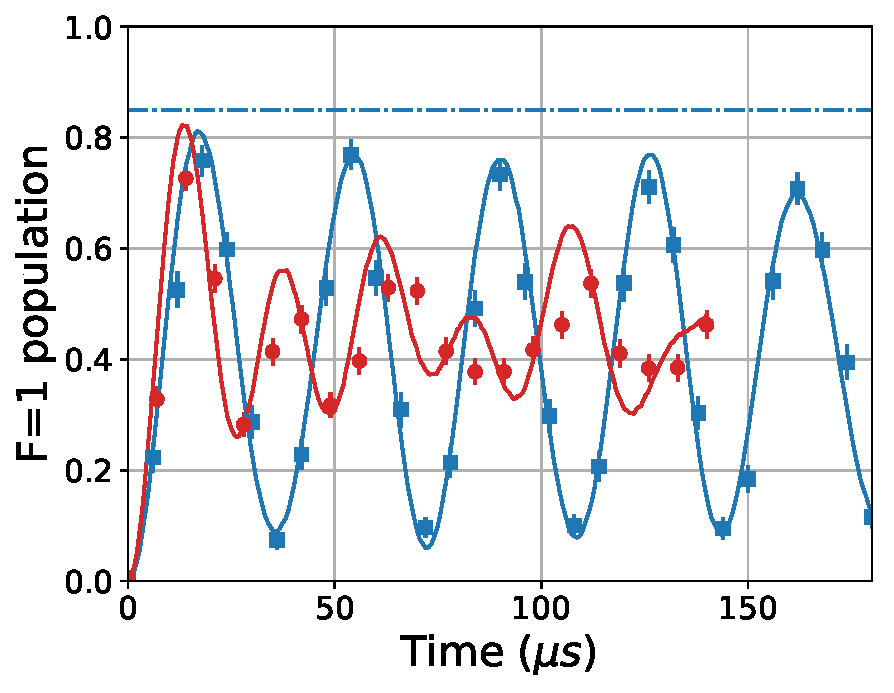
\includegraphics[width=6cm]{imgs/rabi_flop_r2_p1.pdf}};
      \visible<2->{
        \node[below,text width=10cm,align=center] at (3, -1)
        {Good agreement in ground state probability\\between spectrum and Rabi flopping data.};
      }
    \end{tikzpicture}
  \end{center}
\end{frame}

\begin{frame}{Rabi flopping (axial)}
  \begin{center}
    \begin{tikzpicture}
      \node[above] at (0, 0) {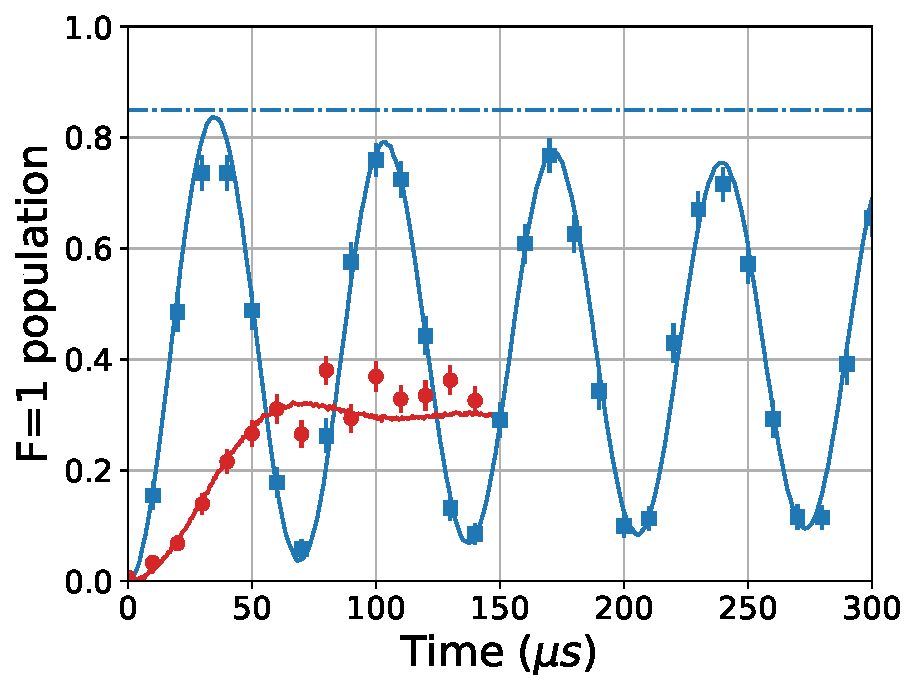
\includegraphics[width=6cm]{imgs/rabi_flop_a1_0.pdf}};
      \node[above] at (6, 0) {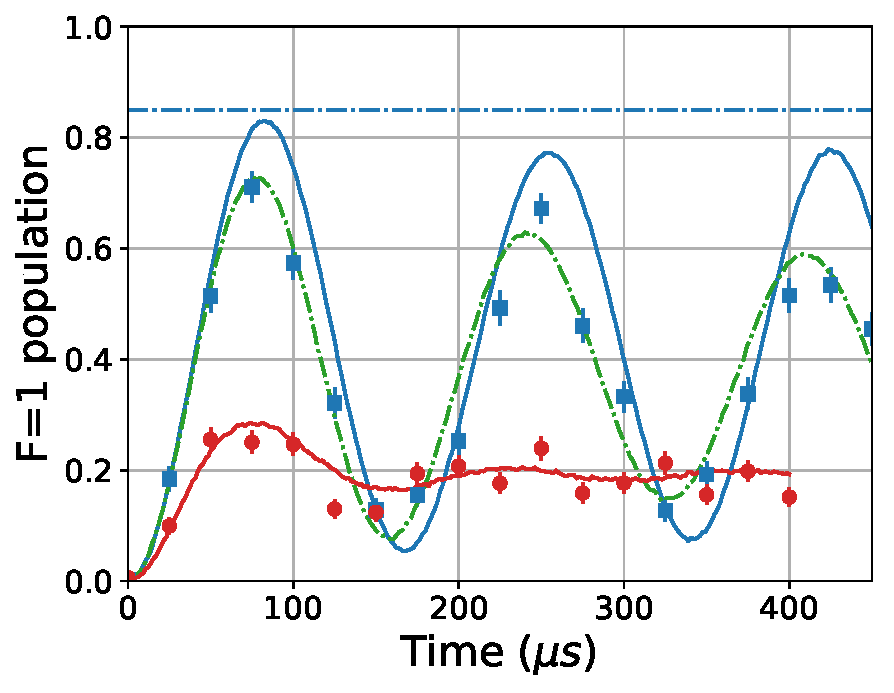
\includegraphics[width=6cm]{imgs/rabi_flop_a1_p1.pdf}};
      \node[below,text width=9cm,align=center] at (3, -1)
      {Decoherence caused by technical noise.\\E.g. $1.5$ mG of magnetic field noise.};
    \end{tikzpicture}
  \end{center}
\end{frame}

% Next step
% * Merge
% * Transfer
\begin{frame}{}
  \hypertarget{conclusion}{}
  \begin{block}{Conclusion}
    \begin{itemize}
    \item Trapping of Na and Cs atoms
    \item Ground state cooling of Na\sfcite{Yu2017} and Cs
    \end{itemize}
  \end{block}
  \begin{block}{In progress}
    \begin{itemize}
    \item \hyperlink{merge-trap-plan}{Merge trap}
    \item \hyperlink{backup-associate}{Photoassociation spectroscopy}
    \item \hyperlink{backup-associate}{Make molecules}
    \end{itemize}
  \end{block}
\end{frame}

\begin{frame}{}
\end{frame}

\begin{frame}{}
\end{frame}

\begin{frame}{}
  \hypertarget<1>{backup-many-body-echo}{}
  \begin{center}
    \hyperlink{applications-many-body}{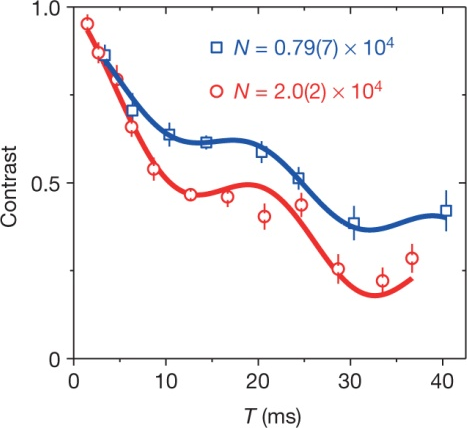
\includegraphics[width=4cm]{imgs/many-body-oscillation.png}}\\
    \visible<3->{
      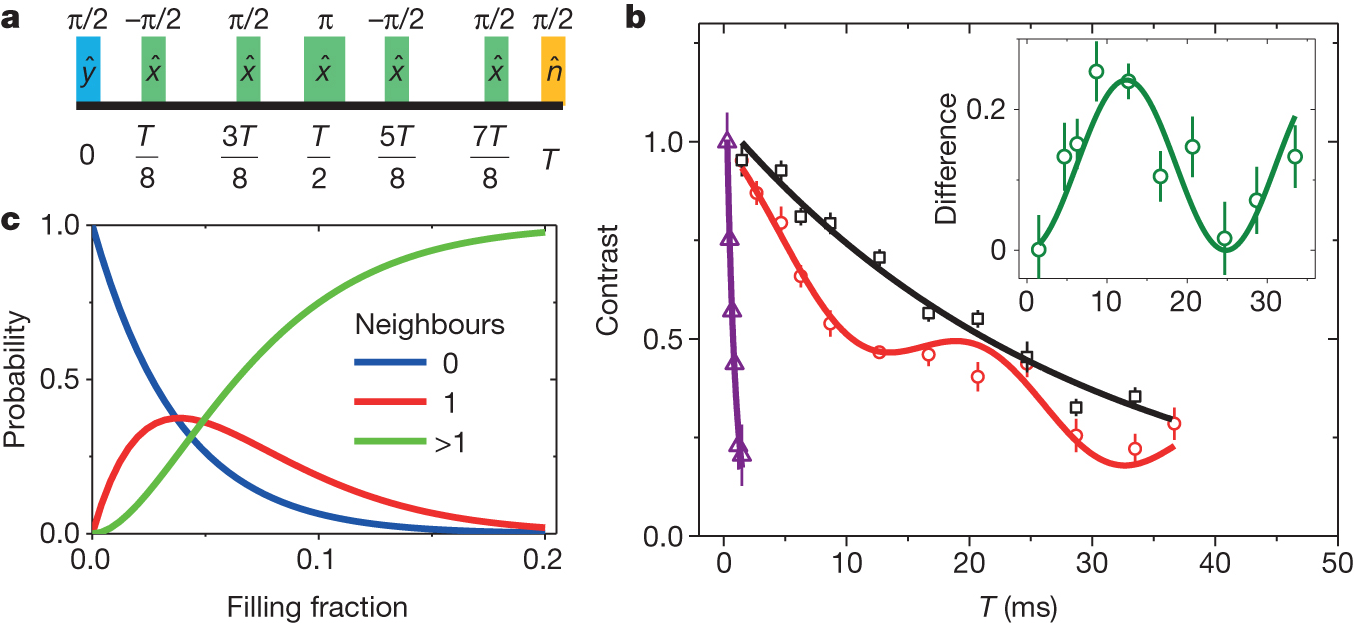
\includegraphics[width=10cm]{imgs/many-body-echo.png}
    }
  \end{center}
\end{frame}

\begin{frame}{}
\end{frame}

\newcommand\drawLevels[1]{
  \draw[line width=1] (#1-0.6, 4.5) -- (#1+0.6, 4.5);
  \draw[line width=1] (#1-0.6, 0) -- (#1+0.6, 0);
  \draw[line width=1] (#1-0.6, -1) -- (#1+0.6, -1);
}

\begin{frame}{\hyperlink{applications-quantum-gate}{Quantum computation}}
  \hypertarget<1>{backup-quantum-gate}{}
  \begin{center}
    \begin{tikzpicture}
      \def\oneColor{yellow!80!black}
      \def\zeroColor{magenta!65!black}
      \node[left] at (-0.6, -1) {\large $|0\rangle$};
      \node[left] at (-0.6, 0) {\large $|1\rangle$};
      \drawLevels{0};
      \drawLevels{2.2};
      \fill [\oneColor,path fading=glow2 fading] (0, 0) circle (0.2);
      \fill [\zeroColor,path fading=glow2 fading] (0, -1) circle (0.2);
      \fill [\oneColor,path fading=glow2 fading] (2.2, 0) circle (0.2);
      \fill [\zeroColor,path fading=glow2 fading] (2.2, -1) circle (0.2);

      \node at (3.5 + 1.1, 4.5) {\hyperlink{backup-exchange-term}{Strong dipole}};
      \node at (3.5 + 1.1, -0.5) {Weak dipole};

      \visible<2->{
        \drawLevels{7};
        \drawLevels{9.2};
        \fill [\oneColor,path fading=glow2 fading] (7, 4.5) circle (0.2);
        \fill [\zeroColor,path fading=glow2 fading] (7, -1) circle (0.2);
        \fill [\oneColor,path fading=glow2 fading] (9.2, 4.5) circle (0.2);
        \fill [\zeroColor,path fading=glow2 fading] (9.2, -1) circle (0.2);

        \draw[-{Stealth[length=10mm, width=5mm]},line width=4,color=red!20!gray]
        plot[domain={-3.5}:{3.5}, variable=\x] ({\x + 3.5 + 1.1}, {5.5 - (\x)^2 / 20});
      }

      \visible<3->{
        \draw[{Stealth[length=10mm, width=5mm]}-,line width=4,color=blue!20!gray]
        plot[domain={-3.5}:{3.5}, variable=\x] ({\x + 3.5 + 1.1}, {-2 + (\x)^2 / 20});
      }
    \end{tikzpicture}
  \end{center}
\end{frame}

\begin{frame}{}
\end{frame}

\begin{frame}{\hyperlink{applications-quantum-gate}{Quantum computation}}
  \hypertarget<1>{backup-exchange-term}{}
  \begin{center}
    \begin{tikzpicture}
      \draw (0, 0.2) -- (0.5, 0.2);
      \draw (0.7, 0.2) -- (1.2, 0.2);
      \draw (0, 1.41) -- (0.5, 1.41);
      \draw (0.7, 1.41) -- (1.2, 1.41);

      \fill [green!80!black,path fading=glow2 fading] (0.25, 0.2) circle (0.1);
      \fill [red!80!black,path fading=glow2 fading] (0.95, 1.41) circle (0.1);

      \draw (0 + 2.0, 0.2) -- (0.5 + 2.0, 0.2);
      \draw (0.7 + 2.0, 0.2) -- (1.2 + 2.0, 0.2);
      \draw (0 + 2.0, 1.41) -- (0.5 + 2.0, 1.41);
      \draw (0.7 + 2.0, 1.41) -- (1.2 + 2.0, 1.41);

      \fill [red!80!black,path fading=glow2 fading] (0.25 + 2.0, 1.41) circle (0.1);
      \fill [green!80!black,path fading=glow2 fading] (0.95 + 2.0, 0.2) circle (0.1);

      \node at (0.6, -1) {\hyperlink{backup-quantum-gate}{\LARGE $E$}};
      \node at (0.6 + 2.0, -1) {\LARGE $\displaystyle\frac{V}{r^3}$};
      \node at (0.6, -1 - 2.0) {\LARGE $\displaystyle\frac{V}{r^3}$};
      \node at (0.6 + 2.0, -1 - 2.0) {\LARGE $E$};

      \node[left] at (0, -1 - 2.0 / 2) {$\left(\vphantom{\rule{1pt}{2.0cm}}\right.$};
      \node[right] at (1.2 + 2.0, -1 - 2.0 / 2) {$\left.\vphantom{\rule{1pt}{2.0cm}}\right)$};

      \visible<2->{
        \draw[-{Stealth[length=10mm, width=8mm]},line width=10,color=blue!20!gray]
        (4, -1 - 2.0 / 2) -- (6.0, -1 - 2.0 / 2);

        \node at (0.6 + 6.6, -1) {\LARGE $\displaystyle E - \frac{V}{r^3}$};
        \node at (0.6 + 2.0 + 6.6, -1 - 2.0) {\LARGE $\displaystyle E + \frac{V}{r^3}$};

        \node[left] at (0 + 6.6, -1 - 2.0 / 2) {$\left(\vphantom{\rule{1pt}{2.0cm}}\right.$};
        \node[right] at (1.2 + 2.0 + 6.6, -1 - 2.0 / 2) {$\left.\vphantom{\rule{1pt}{2.0cm}}\right)$};
      }
    \end{tikzpicture}
  \end{center}
\end{frame}

\begin{frame}{}
\end{frame}

\begin{frame}{}
  \hypertarget{backup-diff-adiabatic}{}
  \begin{center}
    \begin{tikzpicture}
      \node[above] at (-5.5, 0) {\hyperlink{raman-difficulty-pdf}{Before cooling}};
      \node[below] at (-5.5, 0) {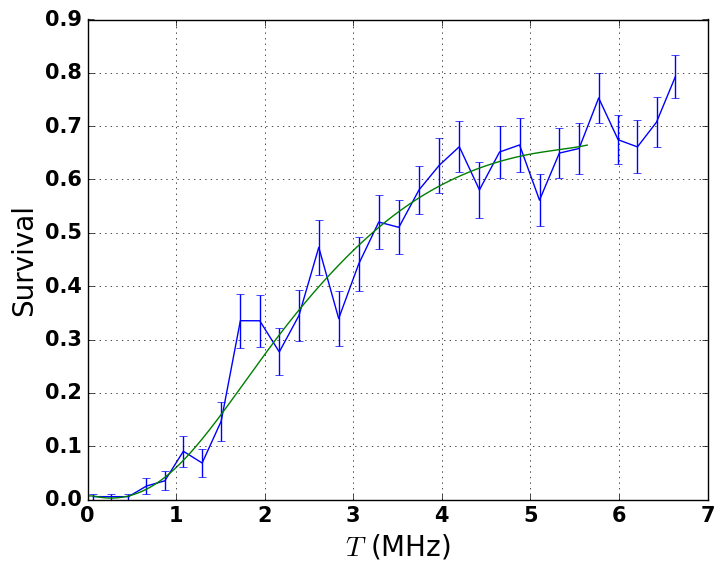
\includegraphics[width=5.2cm]{../../experiments/adiabatic_lowering/imgs/AC_none_cdf.png}};
      \node[below] at (-5.5, -4) {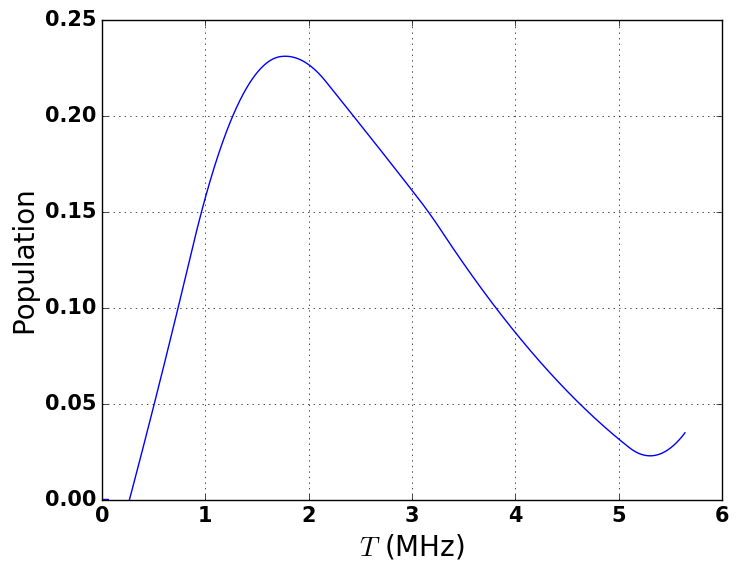
\includegraphics[width=5.2cm]{../../experiments/adiabatic_lowering/imgs/AC_none_pdf.png}};
      \node[above] at (0, 0) {After cooling};
      \node[below] at (0, 0) {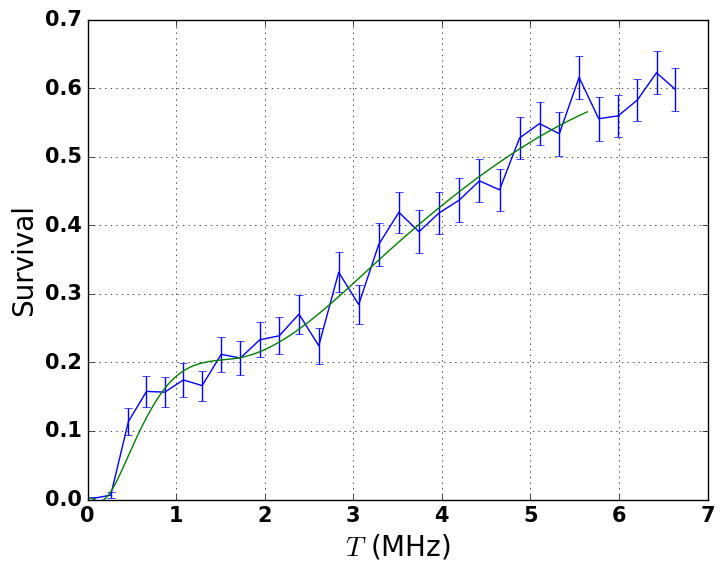
\includegraphics[width=5.2cm]{../../experiments/adiabatic_lowering/imgs/AC_old-pulsed_cdf.png}};
      \node[below] at (0, -4) {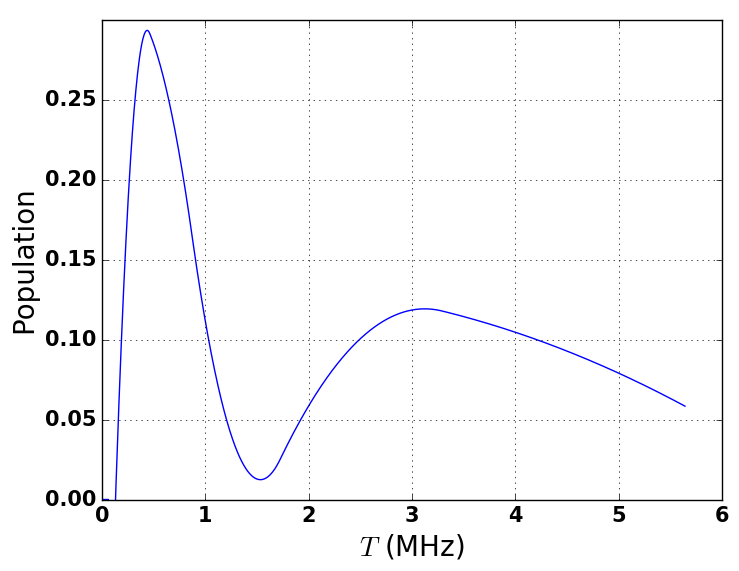
\includegraphics[width=5.2cm]{../../experiments/adiabatic_lowering/imgs/AC_old-pulsed_pdf.png}};
    \end{tikzpicture}
  \end{center}
\end{frame}

\begin{frame}{}
\end{frame}

\begin{frame}{\hyperlink{making-molecule-merge-trap}{Merge} \hyperlink{conclusion}{trap}}
  \hypertarget{merge-trap-plan}{}
  \begin{center}
    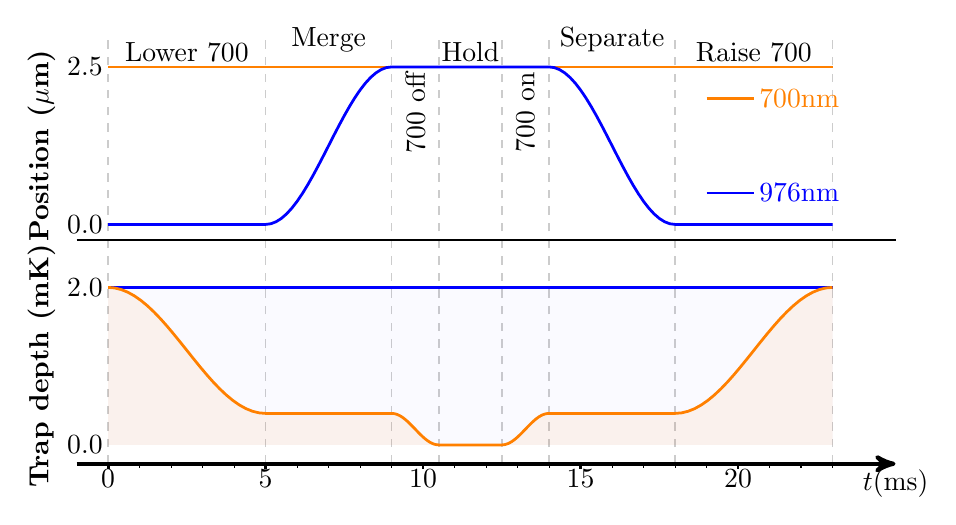
\begin{tikzpicture}[scale=4]
      \def\yoffset{-0.06}
      \foreach \i in {0,0.5,0.9,1.05,1.25,1.4,1.8,2.3} {
        \draw[gray!40,dashed,line width=0.5] (\i, \yoffset) -- (\i, 1.3);
      }
      \draw[line width=1.5,->] (-0.1, \yoffset) -- (2.5, \yoffset) node[below] {$t$(ms)};
      \foreach \i in {0,5,...,20} {
        \draw[line width=1] (\i/10,\yoffset) -- (\i/10,\yoffset-0.015);
        \path (\i/10, \yoffset) node[below] {$\i$};
      }
      \foreach \i in {0,...,23} {
        \draw[line width=0.4] (\i/10,\yoffset) -- (\i/10,\yoffset-0.014);
      }

      \draw[line width=1,blue] (0, 0.5) -- (2.3, 0.5);
      \fill[blue, opacity=0.02] (0, 0) -- (0, 0.5) -- (2.3, 0.5) -- (2.3, 0) -- cycle;
      \draw[line width=1,orange]
      plot[domain={0}:{180},variable=\x] ({\x/180*0.5}, {(cos(\x)+1) / 5 + 0.1})
      -- (0.9, 0.1)
      plot[domain={0}:{180},variable=\x] ({\x/180*0.15 + 0.9}, {(cos(\x)+1) / 2 * 0.1})
      -- (1.25, 0)
      plot[domain={0}:{180},variable=\x] ({\x/180*0.15 + 1.25}, {(1-cos(\x)) / 2 * 0.1})
      -- (1.8, 0.1)
      plot[domain={0}:{180},variable=\x] ({\x/180*0.5 + 1.8}, {(1-cos(\x)) / 5 + 0.1});
      \fill[orange, opacity=0.07] (0, 0)
      -- plot[domain={0}:{180},variable=\x] ({\x/180*0.5}, {(cos(\x)+1) / 5 + 0.1})
      -- (0.9, 0.1)
      -- plot[domain={0}:{180},variable=\x] ({\x/180*0.15 + 0.9}, {(cos(\x)+1) / 2 * 0.1})
      -- (1.25, 0)
      -- plot[domain={0}:{180},variable=\x] ({\x/180*0.15 + 1.25}, {(1-cos(\x)) / 2 * 0.1})
      -- (1.8, 0.1)
      -- plot[domain={0}:{180},variable=\x] ({\x/180*0.5 + 1.8}, {(1-cos(\x)) / 5 + 0.1})
      -- (2.3, 0) -- cycle;

      \draw[line width=0.5] (-0.1, 0.65) -- (2.5, 0.65);
      \draw[line width=1,orange] (0, 1.2) -- (2.3, 1.2);
      \draw[line width=1,blue] (0, 0.7) -- (0.5, 0.7)
      plot[domain={0}:{180},variable=\x] ({\x/180*0.4 + 0.5}, {(1-cos(\x)) / 2 * 0.5 + 0.7})
      -- (1.4, 1.2)
      plot[domain={0}:{180},variable=\x] ({\x/180*0.4 + 1.4}, {(1+cos(\x)) / 2 * 0.5 + 0.7})
      -- (2.3, 0.7);
      \draw[line width=1,orange] (1.9, 1.1) -- (2.05, 1.1) node[right] {$700$nm};
      \draw[line width=1,blue] (1.9, 0.8) -- (2.05, 0.8) node[right] {$976$nm};

      \path (0, 0.0) node[left] {$0.0$};
      \path (0, 0.5) node[left] {$2.0$};
      \path (0, 0.7) node[left] {$0.0$};
      \path (0, 1.2) node[left] {$2.5$};
      \path (-0.15, 0.25) node[above,rotate=90] {\textbf{Trap depth (mK)}};
      \path (-0.15, 0.95) node[above,rotate=90] {\textbf{Position ($\mu$m)}};
      \path (0.25, 1.2) node[above] {Lower $700$};
      \path (0.7, 1.23) node[above] {Merge};
      \path (0.975, 1.2) node[left,rotate=90] {$700$ off};
      \path (1.15, 1.2) node[above] {Hold};
      \path (1.325, 1.2) node[left,rotate=90] {$700$ on};
      \path (1.6, 1.23) node[above] {Separate};
      \path (2.05, 1.2) node[above] {Raise $700$};
    \end{tikzpicture}
  \end{center}
\end{frame}

\begin{frame}{}
\end{frame}

\begin{frame}{\hyperlink{making-molecule-making-molecule}{Making molecule}}
  \hypertarget{backup-associate}{}
  \begin{center}
    \hyperlink{conclusion}{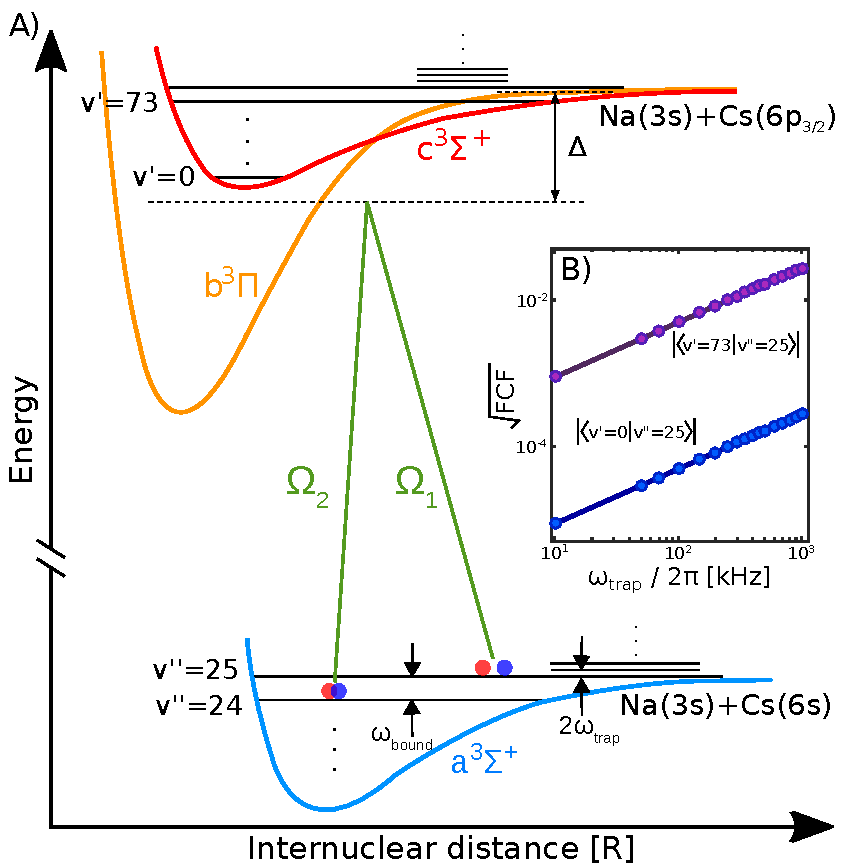
\includegraphics[height=7cm]{imgs/molecule-formation.pdf}}
  \end{center}
\end{frame}

\end{document}
